% !TeX encoding = UTF-8
% !TeX spellcheck = zh-cmn-Hans-CN
% !TeX program = xelatex
% !TeX root = ../main.tex

\documentclass[../main.tex]{subfiles}

\begin{document}
\chapter{测度论}
本章我们将回顾一些测度论当中的一些定义与结论。如果读者没有接触过相关概念,那么可以将本章作为入门材料;如果读者已经有了相关知识,那么可以借本章做知识回顾之用。
一些比较困难的证明,特别是那些不符合直觉的,会放在附录中供读者参考。
如果读者拥有扎实的测度论基础,那么可以跳过\ref{sec:1.4}、\ref{sec:1.5}和\ref{sec:1.7}节,因为这些内容曾经是附录的一部分。

\section{概率空间} \label{sec:1.1}
书中的术语将以\textbf{粗体}标出。我们将从最基本的部分开始。
\term{概率空间}(probability space)是由表示``试验结果''的集合\(\Omega\) 、表示``事件''的集合\(\mathcal{F}\)和一个负责给事件分配概率的函数\(P:\mathcal{F} \rightarrow \intcc{0, 1}\)构成的三元组\((\Omega, \mathcal{F}, \probP)\)。
我们假定\(\mathcal{F}\)是一个\term{\(\sigma\)域}(\(\sigma\)-field)(又称\term{\(\sigma\)代数}(\(\sigma\)-algebra))\footnote{书中会根据语境将两者混用},是\(\Omega\)的(非空)子集族,并满足下列条件:
\begin{enumerate}
	\item \(A \in \mathcal{F} \Rightarrow A^c \in \mathcal{F}\)。
	\item \label{def:measure:2} 如果\(A_i \in \mathcal{F}\)是一个由可数个集合构成的集合列,那么\(\bigcup_i A_i \in \mathcal{F}\)。
\end{enumerate}

此处以及后文当中的\term{可数}(countable)表示基数为有限或可数无穷。由于\(\bigcap_i A_i = (\bigcup_i A_i^c)^c\),因此\(\sigma\)域在可数交下封闭。因此我们在定义中略去了该条性质以便简化验证\(\sigma\)域的过程。

如果没有\(P\),我们称\((\Omega, \mathcal{F})\)为\term{可测空间}(measurable space),即我们可以为该空间中指派一个测度。而\term{测度}(measure)是指非负的加性集函数,即符合下列条件的函数\(\mu: \mathcal{F} \rightarrow \R\)
\begin{enumerate}
	\item \(\forall A \in \mathcal{F}, \mu(A) \geq \mu(\emptyset) = 0\)
	\item 如果\(A_i \in \mathcal{F}\)是一个由可数个互不相交的集合构成的集合列,我们有
	\[\mu\left(\bigcup_i A_i\right) = \sum_{i}\mu(A_i)\]
	如果\(\mu(\Omega) = 1\),我们称这个\(\mu\)为\term{概率测度}(probability measure)。本书通常用\(P\)来表示概率测度。

	下面我们会从测度的定义出发推导一些在后文中常用结果。我们均认为下面提到的集合来自\(\mathcal{F}\)。
	\begin{theorem} \label{thm:1.1.1}
		令\(\mu\)为\((\Omega, \mathcal{F})\)上的测度
		\begin{enumerate}
			\item \label{prop:measure:monotone} \textbf{单调性} 如果 \(A \subseteq B\),那么\(\mu(A) \leq \mu(B)\)。
			\item \textbf{可数次可加性}\label{thm:1.1.1.2} 如果\(A \in \bigcup_{m=1}^\infty A_m\),那么\(\mu(A) \leq \sum_{m=1}^\infty\mu(A_m)\)。
			\item \label{prop:measure:below_continuity} \textbf{下连续性} % TODO: 这个翻译不好
			 如果集列\(\sequence{A}_{i=1}\)满足\(\lim\limits_{i\uparrow+\infty}A_i \stackrel{\uparrow}{=} A\)(即\(A_1 \subseteq A_2 \subseteq \dots\)且 \(\bigcup_i A_i = A\),那么就有 \(\lim\limits_{i\rightarrow+\infty}\mu(A_i) \stackrel{\uparrow}{=} \mu(A)\)。
			\item \textbf{上连续性} 如果集列\(\sequence{A_i}_{i=1}\)满足\(\lim\limits_{i\rightarrow+\infty}A_i \stackrel{\downarrow}{=} A\)(即\(A_1 \supseteq A_2 \supseteq \dots\)且 \(\bigcap_i A_i = A\)且\(\mu(A_1) < \infty\),那么就有 \(\lim\limits_{i\rightarrow+\infty}\mu(A_i) \stackrel{\downarrow}{=} \mu(A)\)。
		\end{enumerate}
	\end{theorem}
	\begin{proof}
		\begin{enumerate}
			\item 用\(B-A = B\cap A^c\)表示二集合的\textbf{差集}。用\(+\)来表示集合的不交并,借助这些记号,我们就可以将\(B\)表示为\(A+(B-A)\),继而有
			\[\mu(B) = \mu(A) + \mu(B-A) \geq \mu(A)\]
			\item 令\(A^\prime_n = A_n \cap A, B_1 = A^\prime_1\),对于\(n > 1\)时,令\(B_n=A^\prime_n - \bigcup_{m=1}^{n-1}A^\prime_m\)
			注意到\(B_n\)互不相交,并且其并为整个\(A\),根据测度定义的性质\ref{def:measure:2}以及本定理的子句\ref{prop:measure:monotone}
			\[\mu(A) = \sum_{m=1}^{+\infty}\mu(B_m) \leq \sum_{m=1}^{+\infty}\mu(A_m)\]
			\item 令\(B_n = A_n - A_{n-1}\),那么\(B_n\)之间互不相交,并且有\(\bigcup_{m=1}^{+\infty} B_m = A, \bigcup_{m=1}^{n} B_m = A_n\),从而
			\[\mu(A) = \sum_{m=1}^{+\infty}\mu(B_m) = \lim\limits_{n\rightarrow +\infty}\bigcup_{m=1}^{n} B_m = \lim\limits_{n\rightarrow +\infty}\mu(A_n)\]
			\item 因为\(A_1 - A_n \uparrow A_1 - A\) 故由本定理的子句\ref{prop:measure:below_continuity}有\(\mu(A_1 - A_n) \uparrow \mu(A_1 - A)\)
			由于\(A_1\supseteq A\),故\(\mu(A_1 - A) = \mu(A_1) - \mu(A)\)从而有结果\(\mu(A_n)\downarrow\mu(A)\)
		\end{enumerate}
	\end{proof}
\end{enumerate}

最简单的例子就是本科概率论中的:
\begin{example}[离散概率空间] \label{ex:1.1.2} 令\(\Omega\)为某个可数集(即有限集或可数无穷集)。令\(\mathcal{F}=2^\Omega\)(即\(\Omega\)的所有子集之集)。并令
\[P(A) = \sum_{\omega \in A} p(\omega), \text{ 其中 } p(\omega) \geq 0 \text{ 且 } \sum_{\omega \in \Omega} p(\omega) = 1\]
我们不难发这个式子其实给出了离散概率空间上一般形式的概率测度。
在许多情形下\(\Omega\)会是有限集,且\(p(\omega) = 1/|\Omega|\),其中\(|\Omega|\)表示\(\Omega\)的基数。\footnote{中文教材中称这种情形为``古典概型''。}

对于可数集上一般形式的概率测度,有一个具体又简单的例子,就是 astragali\footnote{中国也有类似的东西,一般叫``羊拐''或``嘎拉哈''但用途不同。} ,源自古埃及,是一种用羊距骨制做的骰子。若投掷结果是用顶面朝上,则记为四点;若投掷结果是底面朝上,记为三点;由于骨头的两侧是经过打磨的,就是磨面相对较小,因此会存在磨面朝上的情况,这种情况记为六点;其他情况则记一点。
显然这四种情况的地位是不平等的,因此我们需要\(p_1, p_3, p_4\)和\(p_6\)来描述概率测度\(P\)。
\end{example}

在引入下个定义之前,我们需要先知道一个可以直接由\(\sigma\)-域的定义得到的结果:如果\(\mathcal{F}_i, i\in I\)是一个\(\sigma\)-域,那么\(\bigcap_{i\in I}\mathcal{F}_i\)也是一个\(\sigma\)-域。这里的\(I \neq \emptyset\)是任意指标集(也就是说,其可以为不可数集)。
从这个结果中我们可以知道,如果给定集合\(\Omega\)及其子集族\(\mathcal{A}\),那么存在包含\((\mathcal{A}\)的最小\(\sigma\)-域。我们称这个\(\sigma\)-域为\term{由\(\mathcal{A}\)生成的\(\sigma\)-域},并用记号\(\sigma(\mathcal{A})\)表示。

令\(\R^d\)为向量\((x_1, \dots, x_d), x_1, \dots, x_d\in \R\)构成的集合;\(\mathcal{R}^d\)为\term{博雷尔集},即包含所有\(\R^d\)开集的最小\(\sigma\)-域。当\(d=1\)时,上标通常会被略去。
\begin{example}[实直线上的测度]
	\((\R, \mathcal{R}^d)\)上的测度可以通过具有以下性质的\term{斯蒂尔切斯测度函数}(Stieltjes measure function)\(F\)来定义:
	\begin{enumerate}
		\item \(F\)不减
		\item \(F\)右连续,即\(\lim\limits_{y\downarrow x}F(y) = F(x)\)
	\end{enumerate}
\end{example}

\begin{theorem} \label{thm:1.1.4}
	存在\((\R, \mathcal{R})\)上的测度\(\mu\),使得
	\begin{equation} \label{eq:1.1.1}
		\mu(\intoc{a, b}) = F(b) - F(a)
	\end{equation}
\end{theorem}
若\(F(x) = x\),则称该测度为\term{勒贝格测度}(Lebesgue measure)。

\thmref{thm:1.1.4}的证明之路是漫长而又曲折的,因此我们只在此介绍一下本节当中会用到的一些想法,
而把具体细节放在附录的\ref{sec:a.1}节当中。
本定理之所以用``右闭区间''是因为如果\(b_n \downarrow b\),那么
\[\bigcap_{n} \intoc{a, b_n} = \intoc{a, b}\]
而下一个定理会解释为什么要采用``左开区间''。

如果集族\(\mathcal{S}\)符合:\begin{enumerate*}
	\item 其元素在交下封闭,即\(S, T \in \mathcal{S} \Rightarrow S \cap T \in \mathcal{S}\)
	\item 如果\(S \in \mathcal{S}\),那么\(S^c\)可以表示为由有限个\(\mathcal{S}\)中的不交的元素构成的并
\end{enumerate*},则称\(\mathcal{S}\)为\term{半代数}(semialgebra)。
半代数的一个重要例子是:
\begin{example} \label{ex:1.1.5}
	令\(\mathcal{S}_d\)由空集加上具有如下形式的集合构成:
	\[(a_1, b_1]\times\dots\times \intoc{a_d, b_d} \subseteq \R^d,\ \text{其中} -\infty \leq a_i < b_i \leq +\infty\]
\end{example}
式(\ref{eq:1.1.1})定义了半代数\(\mathcal{S}_1\)上的测度\(\mu\),为了从半代数过渡到\(\sigma\)-代数,我们需要借助一个中间产物。
称\(\Omega\)的子集族\(\mathcal{A}\)为一个\term{集(合)域}(field of sets)(或\term{集合上的代数}(algebra))\footnote{原文仅为field。且后文会混用。},如果\(A, B \in \mathcal{A} \Rightarrow A^c, A \cap B \in \mathcal{A}\)。由于\(A \cap B= (A \cup B)^c\),我们可以立即得到\(A \cap B \in \mathcal{A}\)。\(\sigma\)-域显然是一个集域。反之却不是,下面给出反例:

\begin{example}
	令\(\Omega = \mathbf{Z}\)为整数集。则\(\mathcal{A} = \{A: A \text{或} A^c \text{有限}\}\)是一个集域。
\end{example}

\begin{lemma} \label{lem:1.1.7}
	如果\(\mathcal{S}\)是一个半代数,那么\(\bar{\mathcal{S}} = \{\mathcal{S}\text{中元素的有限不交并}\}\)是一个集域,并称其为\term{由\(\mathcal{S}\)生成的集(合)域}。
\end{lemma}
\begin{proof}
	令\(A = +_i S_i\)以及\(B = +_j T_j\),其中\(+\)表示不交并,且指标集是有限集。我们有\(A \cap B = +_{i,j}S_i \cap T_j \in \bar{\mathcal{S}}\)。同样地,对于补运算,令\(A = +_{i}S_i\),有\(A^c = \bigcap_i S_i^c\),而\(\mathcal{S}\)的定义保证了\(S_i^c \in \mathcal{S}\)。从而\(\bar{\mathcal{S}}\)在交运算下是封闭的。因此\(\bar{\mathcal{S}}\)是一个集域。
\end{proof}

\begin{example}
	令\(\Omega = \R\)及\(\mathcal{S} = \mathcal{S}_1\),\(\mathcal{S}_1\)由空集以及下列形式的集合构成
	\[\bigcup_{i=1}^k \intoc{a_i, b_i}, \text{ 其中} -\infty \leq a_i < b_i \leq +\infty\]
	如果给定\(\mathcal{S}\)上的函数\(\mu\),我们可以通过
	\[\mu(+_{i=1}^{n} A_i) = \sum_{i=1}^{n}\mu(A_i)\]
	将其延拓到\(\bar{\mathcal{S}}\)上。
\end{example}

所谓\term{集(合)域\(\mathcal{A}\)上的测度},就是一个满足下列条件的函数\(\mu\):
\begin{enumerate}
	\item \(\forall A \in \mathcal{A}, \mu(A) \geq \mu(\emptyset) = 0\)
	\item 如果\(A_i \in \mathcal{A}\)互不相交且\emph{它们的并在\(\mathcal{A}\)中},那么
	\[\mu\left(\bigcup_{i=1}^{+\infty} A_i\right) = \sum_{i=1}^{+\infty} \mu(A_i)\]
\end{enumerate}
如果存在集合列\(A_n \in \mathcal{A}\),使得\(\mu(A_i) < +\infty\)且\(\bigcup_n A_n = \Omega\),则称\(\mu\)为\term{\(\sigma\)有限}。
令\(A^\prime_1 = A_1\)且对于\(n \geq 2\),
\[A^\prime_1 = \bigcup_{m=1}^n A_m \quad \text{或} \quad A^\prime_1 = A_n \cap \left(\bigcap_{m=1}^{n-1} A_m^c\right) \in \mathcal{A}\]
因此我们可以不失一般性地假定\(A_n \uparrow \Omega\)或\(A_n\)之间互不相交。

下面的结果将帮助我们把半代数\(\mathcal{S}\)上的测度延拓到它生成的\(\sigma\)代数上,即\(\sigma(\mathcal{S})\)上。
\begin{theorem} \label{thm:1.1.9}
	令\(\mathcal{S}\)为一个半代数并令\(\mu\)为定义在\(\mathcal{S}\)上的函数,且\(\mu(\emptyset) = 0\)。假设\begin{enumerate*}
		\item \label{thm:1.1.9.1} 如果\(S \in \mathcal{S}\)来自于有限个互不相交的\(S_i \in \mathcal{S}\)的并,那么\(\mu(S) = \sum_i \mu(S_i)\)
		\item \label{thm:1.1.9.2} 如果\(S_i, S \in \mathcal{S}\)且\(S = +_{i \geq 1} S_i\),那么\(\mu(S) \leq \sum_{i \geq 1} \allowbreak\mu(S_i)\)
	\end{enumerate*}。那么\(\mu\)有唯一的延拓\(\bar{\mu}\)使得其是\(\bar{\mathcal{S}}\),即由\(\mathcal{S}\)生成的集域,上的测度。
	如果\(\bar{\mu}\)是\(\sigma\)有限的,那么存在唯一的延拓\(\nu\),使得\(\nu\)为\(\sigma(\mathcal{S})\)上的测度。
\end{theorem}
在\ref{thm:1.1.9.2}及其后面的内容中,我们会用\(i \geq 1\)表示可数并,而单个的\(i\)或\(j\)表示有限并。由于本节内容使用了\autoref{thm:1.1.9},因此该定理的证明放在了附录的\ref{sec:a.1}节当中。
为了验证定理中的条件\ref{thm:1.1.9.2}成立,用下面的结论会比较方便:
\begin{lemma} \label{lem:1.1.10}
	假定只有条件\ref{thm:1.1.9.1}成立。
	\begin{enumerate}[label*=(\alph*)]
		\item \label{lem:1.1.10.a} 如果\(A, B_i \in \bar{\mathcal{S}}\)并有\(A = +_{i=1}^n S_i\),那么\(\bar{\mu}(A) = \sum_{i=1}^n \bar{\mu}(B_i)\)。
		\item \label{lem:1.1.10.b} 如果\(A, B_i \subseteq \bar{\mathcal{S}}\)并有\(A = +_{i=1}^n S_i\),那么\(\bar{\mu}(A) \leq \sum_{i=1}^n \bar{\mu}(B_i)\)。
	\end{enumerate}
\end{lemma}
\begin{proof}
	从定义中我们可以得知,如果\(A = +_i B_i\)是由互不相交的\(S_i \in \bar{\mathcal{S}}\)构成的且\(B_i = +_j S_{i,j}\),那么
	\[\bar{\mu}(A) = \sum_{i,j} S_{i,j} = \sum_{i} \bar{\mu}(B_i) \]

	为了证明\ref{lem:1.1.10.b},我们从\(n = 1\)的情况开始,此时\(B_1 = B\)。由于\(B = A + (B \cap A^c)\)且\(B \cap A^c \in \bar{\mathcal{S}}\),所以
	\[\bar{\mu}(A) \leq \bar{\mu}(A) + \bar{\mu}(B \cap A^c) = \bar{\mu}(B)\]
	对于\(n > 1\)的情况,只需令\(F_k = B_1^c \cap \dots \cap B_{k-1}^c \cap B_k^c\),并且我们注意到
	\[\begin{split}
		\bigcup_i B_i &= F_1 + \dots + F_n\\
		A = A \cap \left(\bigcup_i B_i\right) &= (A \cap F_1) + \dots + (A \cap F_n)
	\end{split}\]
	故使用\ref{lem:1.1.10.a}、\(n = 1\)时的\ref{lem:1.1.10.b}并再次使用\ref{lem:1.1.10.a},我们便得到
	\[\bar{\mu}(A) = \sum_{k=1}^n \bar{\mu}(A \cap F_k) \leq \sum_{k=1}^n \bar{\mu}(F_k) = \bar{\mu}\left(\bigcup_i B_i\right)\]
\end{proof}
\begin{proof}[\thmref{thm:1.1.4}的证明]
	令\(\mathcal{S}\)为左开右闭区间\(\intoc{a,b}\),其中\(-\infty \leq a < b \leq +\infty\)。为了定义\(\mathcal{S}\)上的函数\(\mu\),
	我们从下面观察到的结果开始:
	\[F(+\infty) = \lim\limits_{x \uparrow +\infty} F(x)\quad \text{以及}\quad
	F(-\infty) = \lim\limits_{x \downarrow -\infty} F(x)\quad\text{存在}\]
	以及\(F(+\infty) > -\infty\)、\(F(-\infty) < +\infty\),故而当\(-\infty \leq a < b \leq +\infty\)时,\(\mu(\intoc{a, b}) = F(b) - F(a)\)是有意义的。

	如果\(\intoc{a, b} = +_{i=1}^{n}\intoc{a_i, b_i}\),那么我们一定可以重新排列区间相应端点的下标,使得\(a_1 = a, b_n = b\)以及对与\(2 \leq i \leq n\),我们有\(a_i = b_{n-1}\)。
	故\thmref{thm:1.1.9}中的条件\ref{thm:1.1.9.1}成立。
	下面验证条件\ref{thm:1.1.9.2},首先假定\(-\infty < a < b < +\infty\)和\(\intoc{a, b} \subseteq \bigcup_{i \geq 1} \intoc{a_i, b_i}\),其中(可不失一般性地认为)\(-\infty < a_i < b_i < +\infty\)。
	选择\(\delta > 0\)使得\(F(a + \delta) < F(a) + \epsilon\)以及\(\eta_i\)使得
	\[F(b_i + \eta_i) < F(b_i) + \epsilon 2^{-i}\]
	那么我们发现开区间\(\intoo{a_i, b_i + \eta_i}\)覆盖了有界闭区间\(\intcc{a + \delta, b}\),故存在有限子覆盖\(\intoo{\alpha_j, \beta_j}\),其中\(1 \leq j \leq J\)。
	由于\(\intoc{a + \delta, b} \subseteq \bigcup_{j=1}^J \intoo{\alpha_j, \beta_j}\),从\lemref{lem:1.1.10}的子句\ref{lem:1.1.10.b}意味着
	\[F(b) - F(a+\delta) \leq \sum{j=1}^J F(\beta_j) - F(\alpha_j) \leq \sum_{i=1}^{+\infty}(F(b_i+\eta_i) - F(a_i))\]
	根据我们选择的\(\delta\)以及\(\eta_i\),我们有
	\[F(b) - F(a) \leq 2\epsilon + \sum_{i=1}^{+\infty}(F(b_i+\eta_i) - F(a_i))\]
	由于\(\epsilon\)是任取的,故我们证明了当\(-\infty < a < b < +\infty\)时,定理是成立的。
	为了消除最后的障碍,只需注意到如果\(\intoc{a, b} \subseteq \bigcup_i \intoc{a_i, b_i}\)且对于当\(-\infty < A < B < +\infty\)时,有\(\intoc{A, B} \subseteq \intoc{a, b}\),那么我们有
	\[F(B) - F(A) \leq \sum_{i=1}^{+\infty} (F(b_i) - F(a_i))\]
	由于最后的结果对任意有界的\(\intoc{A, B} \subseteq \intoc{a, b}\)成立,故而我们得到了最终的结论。
\end{proof}
\subsubsection*{\(\R^{d}\)上的测度}
我们的下一个目标是将\thmref{thm:1.1.4}推广到\(\R^d\)上。我们首先得明确函数\(F\)需要满足的一些性质。模仿\(d = 1\)的情况,我们容易推断出\(F\)应该满足下列性质:
\begin{enumerate}
	\item \label{def:measure.Rd.1} \(F\)是不减的,即当\(x \leq y\)(意思是\(\forall i, x_i \leq y_i\))时,有\(F(x) \leq F(y)\)。
	\item \label{def:measure.Rd.2} \(F\)右连续,即当\(\lim\limits_{y \downarrow x} F(y) = F(x)\)(这里的\(x \downarrow y\)是指每个\(y_i \downarrow x_i\))。
	\item 如果\(x_n \downarrow -\infty\),即每个坐标分量\(x_i \downarrow -\infty\),那么\(\lim\limits_{n\rightarrow+\infty}F(x_n) = 0\)。
	如果\(x_n \uparrow -\infty\),即每个坐标分量\(x_i \uparrow +\infty\),那么\(\lim\limits_{n\rightarrow+\infty}F(x_n) = 1\)。
\end{enumerate}
但是此时情况却变了。考虑如下的\(F:\ \R^2 \mapsto \intcc{0, 1}\)
\[F(x_1, x_2) = \begin{cases}
	1 & \text{若}x_1, x_2 \geq 1\\
	\frac{2}{3} & \text{若}x_1 \geq 1 \text{且} 0 \leq x_2 < 1\\
	\frac{2}{3} & \text{若}x_2 \geq 1 \text{且} 0 \leq x_1 < 1\\
	0 & \text{其他}\\
\end{cases}\]
\begin{figure}
\centering
\begin{tikzpicture}[scale=2]
	\begin{scope}
		% probabilities
		\draw (.5,.5) node[anchor=base] {\huge $0$};
		\draw (-.5,.5) node[anchor=base] {\huge $0$};
		\draw (.5,-.5) node[anchor=base] {\huge $0$};
		\draw (-.5,1.5) node[anchor=base] {\huge $0$};
		\draw (1.5,-.5) node[anchor=base] {\huge $0$};
		\draw (-.5,-.5) node[anchor=base] {\huge $0$};
		\draw (1.5,.5) node[anchor=base] {\huge $\frac{2}{3}$};
		\draw (.5,1.5) node[anchor=base] {\huge $\frac{2}{3}$};
		\draw (1.5,1.5) node[anchor=base] {\huge $1$};

		% ticks
		\draw[xshift=1 cm,dashed] (0,2.2) -- (0,-1.2) node[below] {};
		\draw[yshift=1 cm, dashed] (2.2,0) -- (-1.2,0) node[left] {};
		\draw (1,0) node[anchor=north east] {$1$};
		\draw (0,1) node[anchor=north east] {$1$};

		% origin
		\draw (0,0) node[anchor=north east] {\Large $O$};

		% axes
		\draw[thick,->] (-1.2,0) -- (2.2, 0) node[below] {\Large $x_1$};
		\draw[thick,->] (0,-1.2) -- (0, 2.2) node[left] {\Large $x_2$};
	\end{scope}
\end{tikzpicture}
\caption{反例的示意图}
\label{fig:1.1}
\end{figure}
\figref{fig:1.1}给出了该反例的图像。
如果稍加思索,我们可以知道
\[\begin{split}
	\mu(\intoc{a_1, b_1} \times \intoc{a_2, b_2}) = &\mu(\intoc{-\infty,b_1} \times \intoc{-\infty,b_2}) - \mu(\intoc{-\infty,a_1} \times \intoc{-\infty,b_2})\\
&-\mu(\intoc{-\infty,b_1} \times \intoc{-\infty,a_2}) + \mu(\intoc{-\infty,a_1} \times \intoc{-\infty,a_2})\\
=&F(b_1, b_2) - F(a_1, b_2) - F(b_1, a_2) + F(a_1, a_2)
\end{split}\]
令\(\epsilon \rightarrow 0\), 把\(a_1=a_2=1-\epsilon\)和\(b_1=b_2=1\)带入上式,我们会发现
\[\mu(\intcc{1,1} = 1-\frac{2}{3}) - \frac{2}{3} + 0 = -\frac{1}{3}\]
用同样的方法,我们可以得到\(\mu(\intcc{1,0}) = \mu(\intcc{0,1})=2/3\)。

为了得到使\(F\)成为测度的第三个也是最后一个条件,令
\[\begin{split}
	A &= \intoc{a_1, b_1}\times\dots\times\intoc{a_d,b_d}\\
	V &= \{a_1, b_1\}\times\dots\times\{a_d,b_d\}
\end{split}\]
其中\(-\infty < a_i < b_i < +\infty\)。为了强调\(\infty\)不会出现在端点,我们称\(A\)为一个有限矩形。那么\(V\)就是矩形\(A\)的端点集。如果\(v \in V\),令
\[\begin{split}
	\sgn(v) &= (-1)^{v\text{中}a_i\text{的个数}}\\
	\Delta_A F &= \sum_{v \in V} \sgn(v)F(v)
\end{split}\]
若我们要让\(\mu(A) = \Delta_A F\),我们必须要假定
\begin{enumerate}
	\setcounter{enumi}{3}
	\item \label{def:measure.Rd.4} 对所有的矩形\(A\),\(\Delta_A F \geq 0\)。
\end{enumerate}

\begin{theorem} \label{thm:1.1.11}
	假设\(F:\ \R^d \mapsto \intcc{0,1}\)满足条件\ref{def:measure.Rd.1}--\ref{def:measure.Rd.4}。
	那么\(\R^d, \mathcal{R}^d\)上存在唯一的测度\(\mu\),使得对于所有的有限矩形\(A\),有\(\mu(A) = \Delta_A F\)。
\end{theorem}

\begin{example}
	假设\(F(x) = \prod_{i=1}^{d}(F_i(x_i))\),其中\(F_i\)满足\thmref{thm:1.1.4}的条件\ref{def:measure.Rd.1}和条件\ref{def:measure.Rd.2}。
	此时,\[\Delta_A F = \prod_{i=1}^{d}(F_i(b_i) - F_i(a_i))\]
	当\(F_i(x) = x\)时,称该测度为\(\R^d\)上的勒贝格测度。
\end{example}
\begin{proof}
	令\(\mu(A) = \Delta_A F\)对所有有限矩形成立,然后利用单调性将其延拓到\(\mathcal{S}^d\)上。
	为了验证\thmref{thm:1.1.9}的条件\ref{thm:1.1.9.1},我们先引入一些概念。若点列符合\(a_i = \alpha_{i,0} < \alpha_{i,1} \dots < \alpha_{i,n} = b_i\)使得每个\(B_k\)可表示为
	\[\intoc{\alpha_{1,j_1-1, \alpha_{1,j_1}}} \times \dots \times \intoc{\alpha_{d, j_d-1},j_d}\quad \text{其中 } 1\leq j_i \leq n_i\]
	,则称\(A = +_k B_k\)为\(A\)的\term{正则细分}(regular subdivision)。
	容易看到,对于正则细分\(\lambda(A) = \sum_{k}\lambda(B_k)\)。(首先考虑所有断点是有限的情况,然后再将断点取极限就得到了一般结果。)
	为了将该结果推广到一般的有限细分\(A = +_j A_j\)上,只要将每个子矩形进行正则细分即可,这样我们就得到了\(A\)的正则细分。

	条件\ref{def:measure.Rd.2}的证明和\thmref{thm:1.1.4}如出一辙。为了保证与\thmref{thm:1.1.4}之证明记号的一致性\footnote{为了不与下标混淆,这里对于开覆盖取了上标。},对于\(x,y\in \R^d\),我们可以令
	\[\begin{split}
		\intoo{x,y} &= \intoo{x_1,y_1}\times \dots \times \intoo{x_d,y_d}\\
		\intoc{x,y} &= \intoc{x_1,y_1}\times \dots \times \intoc{x_d,y_d}\\
		\intcc{x,y} &= \intcc{x_1,y_1}\times \dots \times \intcc{x_d,y_d}
	\end{split}\]
	假设\(-\infty < a < b < +\infty\),这意味着每个每个端点都是有限的,并假设\(\intoc{a,b} \subseteq \bigcup_{i \geq 1} \intoc{a^i, b^i}\),其中(我们可以不失一般性地认为)\(-\infty < a^i < b^i < +\infty\)。
	令\(\bar{1} = (1,\dots,1)\),取\(\delta\)使得
	\[\mu(\intoc{a-\delta \bar{1},b}) > \mu(\intoc{a,b})\]
	并取\(\eta_i\)使得
	\[\mu(\intoc{a,b^i+\eta_i\bar{1}}) < \mu(\intoc{a^i, b^i}) + \epsilon 2^{-i}\]
	那么开矩形\(\intoo{a^i, b^i}\)会覆盖有界闭矩形\(\intcc{a+\delta\bar{1},b}\),那么必然存在子覆盖\(\intoo{\alpha^j, \beta^j}\),\(1 \leq j \leq J\)。
	由于\(\intoc{a+\delta\bar{1},b} \subseteq \bigcup_{j=1}^J \intoo{\alpha^j, \beta^j}\),\lemref{lem:1.1.10}的\ref{lem:1.1.10.b}意味着
	\[\mu(\intcc{a+\delta\bar{1},b}) \leq \sum_{j=1}^J \mu(\intoc{\alpha^j, \beta^j}) \leq \sum_{i=1}^{+\infty} \mu(\intoc{a^i, b^i+\eta_i\bar{1}})\]
	根据选择的\(\delta\)与\(\eta_i\)我们有
	\[\mu(\intoc{a,b}) \leq 2\epsilon + \sum_{i=1}^{+\infty} \mu(\intoc{a^i, b^i})\]
	由于\(\epsilon\)是任意的,我们就证明了该定理在\(-\infty < a < b < +\infty\)时的情形。
	为了完成证明,我们只需要重复在\thmref{thm:1.1.4}中的工作即可。
\end{proof}

\begin{figure}
\centering
\begin{tikzpicture}[scale=0.6]
	\begin{scope}
		% square
		\draw (0,0) -- (0,7) -- (7,7) -- (7,0) -- (0,0);

		\draw (0,3) -- (5,3);
		\draw (3,6) -- (5,6);

		\draw (2,0) -- (2,3);
		\draw (3,3) -- (3,7);
		\draw (5,0) -- (5,7);
	\end{scope}
\end{tikzpicture}
\hspace{1cm}

\begin{tikzpicture}[scale=0.6]
	\begin{scope}
		% square
		\draw (0,0) -- (0,7) -- (7,7) -- (7,0) -- (0,0);

		\draw (0,4) -- (7,4);
		\draw (0,3) -- (7,3);
		\draw (0,6) -- (7,6);
		\draw (2,0) -- (2,7);
		\draw (3,0) -- (3,7);
		\draw (5,0) -- (5,7);
	\end{scope}
\end{tikzpicture}
\caption{将细分转化为正则细分}
\end{figure}

\subsection*{习题}
\begin{exercise}
	\item 令\(\Omega = \R, \mathcal{F} = \{A\subseteq \R: A\text{或}A^c \text{可数}\}\)。当\(A\)可数时,\(P(A) = 0\),反之则\(P(A) = 1\)。
	证明\((\Omega, \mathcal{F}, \probP)\)是概率空间。
	\item 回顾\exref{ex:1.1.5}中\(\mathcal{S}_d\)的定义。
	证明\(\sigma(\mathcal{S}_d) = \mathcal{R}^d\),即由\(\R^d\)的博雷尔集构成的集族。
	\item 给定一个\(\sigma\)-域\(\mathcal{F}\),如果存在可数集\(\mathcal{C}\subseteq \mathcal{F}\)使得\(\sigma(\mathcal{C}) = \mathcal{F}\),则称\(\mathcal{F}\)是\term{可数生成的}(countably generated)。
	证明\(\mathcal{R}^d\)是可数生成的。
	\item \begin{enumerate*}
		\item 证明若\(\mathcal{F}_1 \subseteq \mathcal{F}_2 \subseteq \dots\)是\(\sigma\)-代数,则\(\bigcup_i \mathcal{F}_i\)是一个代数
		\item 举例说明\(\bigcup_i \mathcal{F}_i\)不一定是\(\sigma\)-代数。
	\end{enumerate*}
	\item 若对于一个集合\(A \subseteq \mathbf{N}^+\)有
	\[\lim\limits_{n \rightarrow +\infty} \frac{\envert{A \cap \{1,2,\dots,n\}}}{n} = \theta\]
	,则称集合\(A\)有\term{自然密度}(natural density)(又称\term{渐进密度}(asymptotic density))\(\theta\)。
	令\(\mathcal{A}\)是由自然密度存在的集合构成的集族。那么\(\mathcal{A}\)是\(\sigma\)域吗?是集域吗?
\end{exercise}

\section{分布} \label{sec:1.2}
当我们为概率空间定义随机变量的时候,事情会变得有意思起来。如果称定义在\(\Omega\)上的实值函数\(X\)满足\(\forall B\in \mathcal{R}, X^{-1}(B) = \{\omega: X(\omega) \in B\} \in \mathcal{F}\),则称\(X\)为\term{随机变量}(random variable)。有时为了加强\(\sigma\)域的存在感,我们会称\(X\)是\term{\(\mathcal{F}\)可测}的(\(\mathcal{F}\)-measurable)或记为\(X \in \mathcal{F}\)。
如果\(\Omega\)是一个离散概率空间(见\exref{ex:1.1.2}),那么任意函数\(X: \Omega \mapsto \R\)均为随机变量。
另一个平凡但实用的随机变量是集合\(A \in \mathcal{F}\)的\term{指示函数}(indicator function):
\[\indicator_A(\omega) = \begin{cases}
	1 & \omega \in A\\
	0 & \omega \notin A
\end{cases}\]
这个记号的用意是提醒你它会将\(A\)中的元素映为\(1\)。分析学家通常叫它\(A\)的特征函数。不过要说明的是,在概率论中,这个术语被用于称呼另一个完全不同的东西(见\ref{sec:3.3}节)。

\begin{figure}[H]
\centering
\begin{subfigure}{.4\textwidth}
	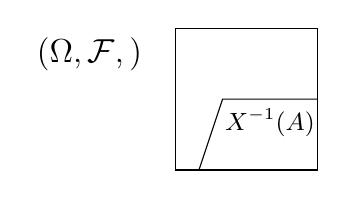
\begin{tikzpicture}[scale=0.3]
		\draw (-1,6) node[anchor=north east] {\large \((\Omega, \mathcal{F}, \probP)\)};
		\draw (0,0) -- (6,0) -- (6,6) -- (0,6) -- (0,0);
		\draw (1,0) -- (2,3) -- (6,3);

		\draw (4,1) node[anchor=south] {\small $X^{-1}(A)$};
	\end{tikzpicture}
\end{subfigure}
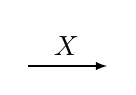
\begin{tikzpicture}
	\draw [-latex](0,0) -- (1,0);
	\node[text width=1em] at (0.5,0.25) {$X$};
\end{tikzpicture}
\begin{subfigure}{.4\textwidth}
	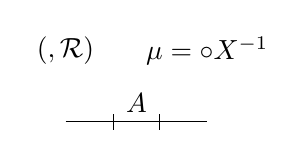
\begin{tikzpicture}[scale=0.3]
		\draw (0,0) -- (2,0);
		\draw [|-|](2,0) -- (4,0);
		\draw (4,0) -- (6,0);

		\draw (3,0) node[anchor=south] {\(A\)};
		\draw (0,2) node[anchor=south] {\((\R, \mathcal{R})\)};
		\draw (6,2) node[anchor=south] {\(\mu = \probP\circ X^{-1}\)};
	\end{tikzpicture}
\end{subfigure}
\caption{\(X\)的分布的定义}
\end{figure}
如果\(X\)是一个随机变量,那么通过对博雷尔集\(A\)定义测度\(\mu(A) = P(X \in A)\)诱导出的在\(\R\)上的概率测度称为\(X\)的\term{分布}(distribution)。
通过之前引入的记号,我们可以将等式右侧写成\(P(X^{-1}(A))\),也就是说我们先通过\(X^{-1}\)将博雷尔集\(A \in \mathcal{R}\)拉回到\(\sigma\)-域上的集合\(X^{-1}(A) \in \mathcal{F}\)上再通过概率测度\(P\)得到相应的概率。

为了验证\(\mu\)是概率测度,我们注意到如果\(A_i\)互不相交,那么通过\(\mu\)的定义,我们就知道\(X\)落在\(A_i\)的并中当且仅当\(X\)落在某个\(A_i\)中;也就是说,如果一组集合\(A_i \in \mathcal{R}\)是互不相交的,那么相应的事件\(\{X \in A_i\}\)也是互不相交的,再次借助\(\mu\)的定义,我们便有
\[\begin{split}
	&\mu\del{\bigcup_{i}A_i} = P\del{X \in \bigcup_{i}A_i}\\ =&P\del{\bigcup_{i} \{X \in A_i\}} = \sum_{i} P(X \in A_i) = \sum_i \mu(A_i)
\end{split}\]
我们一般是通过随机变量\(X\)的\term{分布函数}(distribution function),\(F(x) = P(X \leq x)\),来描述它的分布。

\begin{theorem} \label{thm:1.2.1}
	任何分布函数均有下列性质:
	\begin{enumerate}
		\item \label{thm:1.2.1.1} \(F\)不减。
		\item\label{thm:1.2.1.2} \(\lim\limits_{x \rightarrow +\infty} F(x) = 1\),\(\lim\limits_{x \rightarrow -\infty} F(x) = 0\)。
		\item\label{thm:1.2.1.3} \(F\)右连续,即\(\lim\limits_{y \rightarrow x^+} F(y) = F(x)\)。
		\item\label{thm:1.2.1.4} 若\(F(x^-) = \lim\limits_{y\rightarrow x^-}F(y)\)则\(F(x^-) = \probP(X < x)\)。
		\item\label{thm:1.2.1.5} \(P(X=x) = F(x) - F(x^-)\)。
	\end{enumerate}
\end{theorem}
\begin{proof}
	为了证明\ref{thm:1.2.1.1},只需注意到若\(x \leq y\)则有\(\{X \leq x\} \subseteq \{X \leq y\}\),之后使用\thmref{thm:1.1.1}的子句\ref{prop:measure:monotone}我们就可以得出\(P(X \leq x) \leq P(X \leq y)\)。

	为了证明\ref{thm:1.2.1.2},注意到若\(x \rightarrow +\infty\),则有\(\{X \leq x\} \uparrow \Omega\);同样地,我们还有若\(x \downarrow -\infty\),则有\(\{X \leq x\} \downarrow \emptyset\)。

	为了证明\ref{thm:1.2.1.3}只需注意到若\(y\downarrow x\)则\(\{X \leq y\} \downarrow \{X \leq x\}\)。

	为了证明\ref{thm:1.2.1.4}只需注意到若\(y\uparrow x\)则\(\{X \leq y\} \uparrow \{X \leq x\}\)。

	至于\ref{thm:1.2.1.5},只需注意到\(P(X = x) = P(X \leq x) - P(X < x)\),然后使用\ref{thm:1.2.1.3}和\ref{thm:1.2.1.4}即可。
\end{proof}

下一个结果将为我们进一步地刻画分布函数的性质。

\begin{theorem} \label{thm:1.2.2}
	如果\(F\)符合\thmref{thm:1.2.1}中的\ref{thm:1.2.1.1}、\ref{thm:1.2.1.2}和\ref{thm:1.2.1.3},那么它必然是某个随机变量的分布函数。
\end{theorem}
\begin{proof}
	令\(\Omega = \intoo{0,1}, \mathcal{F}=\Omega\)上的博雷尔集构成的集合,然后令\(P=\)勒贝格测度。对于\(\omega \in \intoo{0,1}\),定义
	\[X(\omega) = \sup\{y:F(y) < \omega\}\]
	如果我们能证明
	\[\tag{$\star$}\label{thm:1.2.2.star}\{\omega: X(\omega) < x\} = \{\omega:\omega\leq F(x)\}\]
	那么我们就可以立即得到想要的结果,因为\(P(\omega:\omega\leq F(x)) = F(x)\)。(因为\(P\)在这里是勒贝格测度。)
	为了验证(\ref{thm:1.2.2.star}),我们注意到如果\(\omega\leq F(x)\),那么就有\(X(\omega) \leq x\),因为\(x \notin \{y: F(y) < \omega\}\)。
	如果\(\omega > F(x)\),从\(F\)的右连续性中可以得出,存在\(\epsilon > 0\)使得\(F(x+\epsilon) < \omega\)以及\(X(\omega) \geq x+\epsilon > x\)。
\end{proof}
\begin{figure}
\centering
\begin{tikzpicture}
	\draw[->] (-1, 0) -- (9, 0) node[right] {\(X\)};
	% \draw[->] (0, 0) -- (0, 1.2) node[left] {\(\probP\)};

	\draw[domain=-2:0, variable=\x, thick] plot ({\x}, {0});
	\draw[domain=0:2, variable=\x, thick] plot ({\x}, {0.5*\x});
	\draw[domain=2:4, variable=\x, thick] plot ({\x}, {0.5*\x+1});
	\draw[domain=4:5, variable=\x, thick] plot ({\x}, {3});
	\draw[domain=5:6, variable=\x, thick] plot ({\x}, {\x-2});
	\draw[domain=6:8, variable=\x, thick] plot ({\x}, {4});
	\draw [fill=white] (2,1) circle [radius=1.5pt];
	\draw [fill=black] (2,2) circle [radius=1.5pt];


	\draw [densely dashed] (-1,1.5)node[left]{\(y\)} -- (2,1.5) -- (2,0)node[below]{\(F^{-1}(x)\)};
	\draw [densely dashed] (-1,3)node[left]{\(y\)} -- (4,3) -- (4,0)node[below]{\(F^{-1}(y)\)};
\end{tikzpicture}
\caption{\thmref{thm:1.2.2}的证明中定义的``逆映射''}
\end{figure}

即便\(F\)不是单射也不是满射(即不是双射),我们还是会称\(X\)为\(F\)的逆,并记为\(F^{-1}\)。
证明\thmref{thm:1.2.2}所用到的方法被广泛应用于计算机中随机变量的生成。
首先生成一个具有均匀分布的随机变量\(U\),然后借助\thmref{thm:1.2.2}中构造的\(F\)来得到一个新的随机变量\(F^{-1}(U)\),显然其分布函数就是\(F\)。

如果\(X\)和\(Y\)在\((\R,\mathcal{R})\)上诱导出了相同的分布\(\mu\),我们就称\(X\)和\(Y\)是\term{在分布意义下相等}(equal in distribution)的。
根据\thmref{thm:1.1.4},\(X\)和\(Y\)在分布意义下相等当且仅当\(X\)和\(Y\)具有相同的分布,人们通常会记为
\[X \stackrel{d}{=} Y\]
但是这个记号在本中显得太长了,出于印刷等方面的因素我们会使用记号\(X =_d Y\)。\footnote{既然是电子版就不搞这些了。}

当一个分布函数\(F(x) = P(X \leq x)\)具有如下形式:
\begin{equation}\label{eq:1.2.1}
	F(x) = \int_{-\infty}^{x}f(y) \dif y
\end{equation}
则称\(X\)具有\term{概率密度函数}(probability density function (PDF))\(f\)。为了便于认知,我们可以认为\(f(x)\)就``代表''了\(P(X=x)\),尽管在实际上
\[P(X = x) = \lim\limits_{\epsilon \rightarrow 0}\int_{x-\epsilon}^{x+\epsilon} f(y) \dif y = 0\]
出于一般性的考量,我们不会使用诸如\(P(X=x)\)的记号来表示密度函数。取而代之的是另一个更具启发意义的记号\(f_X(x)\)。

因此我们可以借助\(f\)和式\eqref{eq:1.2.1}来定义分布函数\(F\)。为了让其结果是分布函数,其充分必要条件为\(f(x) \geq 0\)且\(\int_\R f(x) \dif x = 1\)。
下面展示三个比较重要的例子:
\begin{example}[\(\intoo{0,1}\)上的均匀分布]
	若\(x \in \intoo{0,1}\),则\(f(x) = 1\),其他情况则为\(0\)。
	其分布函数为:
	\[F(x) = \begin{cases}
		0&x\leq 0\\
		x&0\leq x\leq 1\\
		1&x>1
	\end{cases}\]
\end{example}
\begin{example}[率参数为\(\lambda\)的指数分布]
	若\(x \geq 0\)则\(f(x) = \lambda e^{-\lambda x}\)其他情况则为\(0\)。
	其分布函数为
	\[F(x) = \begin{cases}
		0&x\leq 0\\
		1-e^{-\lambda x}&x \geq 0
	\end{cases}\]
\end{example}
\begin{example}[标准正态分布]
	\[f(x) = (2\pi)^{-1/2}\exp(-x^2/2)\]
\end{example}
此时\(F\)并没有所谓的闭合式,但是针对比较大的\(x\),它的分布有如下形式的界:
\begin{theorem} \label{thm:1.2.6}
	对\(x > 0\)
	\[(x^{-1} - x^{-3})\exp(-x^2/2) \leq \int_{x}^{+\infty} \exp(-y^2/2) \dif y \leq x^{-1}\exp(-x^2/2)\]
\end{theorem}
\begin{proof}
	做换元\(y=x+z\)并用不等式\(\exp(-z^2/2) \leq 1\),我们有
	\[\int_{x}^{+\infty} \exp(-y^2/2) \dif y \leq \exp(-x^2/2)\int_{0}^{+\infty}\exp(-xz) \dif z = x^{-1}\exp(-x^2/2)\]
	对于不等式的另一侧,注意到
	\[\int_{x}^{+\infty} (1-3y^{-4})\exp(-y^2/2) \dif y = (x^{-1} - x^{-3})\exp(-x^2/2)\]
\end{proof}
如果一个\(\R\)上的分布函数具有概率密度函数,则称该分布是绝对连续的;如果其分布函数对应的测度较勒贝格测度是奇异的,则称该分布是奇异的。有关这些记号的更多内容请参考\secref{sec:a.4}。
一个奇异分布的例子是:
\begin{example}[康托尔集上的均匀分布]\label{ex:1.2.7}
我们通过如下方式构造康托尔集\(C\):去掉\(\intcc{0,1}\)中间的三分之一\(\intoo{1/3,2/3}\),之后对剩余区间不断重复此过程。
现在定义与之关联的分布函数\(F(x)\),当\(x\leq0\)时\(F(x)=0\),当\(x\geq1\)时\(F(x)=1\),当\(x\in\intcc{1/3,2/3}\)时\(F(x)=1/2\),当\(x\in\intcc{1/9,2/9}\)时\(F(x)=1/4\),当\(x\in\intcc{7/9,8/9}\)时\(F(x)=3/4\)……之后借助单调性将其延拓到整个\(\intcc{0,1}\)上。
此时不存在\(f\)使得\eqref{eq:1.2.1}成立,因为如果\(f\)存在的话它必须在一个测度为\(1\)的集合上等于\(0\)。根据康托尔集的定义,\(\mu(\intcc{0,1}\backslash C)=0\)。
\end{example}
\begin{figure}
\centering
\tikzset{
	if/.code n args=3{\pgfmathparse{#1}\ifnum\pgfmathresult=0
		\pgfkeysalso{#3}\else\pgfkeysalso{#2}\fi},
	lower cantor/.initial=.3333, upper cantor/.initial=.6667, y cantor/.initial=.5,
	declare function={
		cantor_l(\lowerBound,\upperBound)=
		(\pgfkeysvalueof{/tikz/lower\space cantor})*(\upperBound-\lowerBound)+\lowerBound;
		cantor_u(\lowerBound,\upperBound)=
		(\pgfkeysvalueof{/tikz/upper\space cantor})*(\upperBound-\lowerBound)+\lowerBound;
		cantor(\lowerBound,\upperBound)=% fun definition
		(\pgfkeysvalueof{/tikz/y\space cantor})*(\upperBound-\lowerBound)+\lowerBound;},
	cantor start/.style n args=5{%
		insert path={(#1,#3)},
		cantor={#1}{#2}{#3}{#4}{#5}{0},
		insert path={to[every cantor edge/.try, cantor 1 edge/.try] (#2,#4)}},
	cantor/.style n args=6{%
		/utils/exec=%
		\pgfmathsetmacro\lBx{cantor_l(#1,#2)}%
		\pgfmathsetmacro\uBx{cantor_u(#1,#2)}%
		%      \pgfmathsetmacro\y{.5*(#3+#4)},% proper definition
		\pgfmathsetmacro\y{cantor(#3,#4)},% fun
		style/.expanded={
			if={#6<#5}{cantor={#1}{\lBx}{#3}{\y}{#5}{#6+1}}{},
			insert path={
				to[every cantor edge/.try, cantor 1 edge/.try] (\lBx,\y)
				to[every cantor edge/.try, cantor 2 edge/.try] (\uBx,\y)},
			if={#6<#5}{cantor={\uBx}{#2}{\y}{#4}{#5}{#6+1}}{}}}}

	\begin{tikzpicture}[line join=round]
		\draw[thick, cantor start={0}{6}{0}{6}{5}{0}];
		\draw[|-|] (0,0) node[below]{\(0\)} -- (6,0)node[below]{\(1\)};
	\end{tikzpicture}
\caption{康托尔分布}
\end{figure}

\begin{example}[\(0\)处的单点分布]
	\[F(x)=\begin{cases}
		1,\quad x\geq0\\
		0,\quad x<0
	\end{cases}\]
\end{example}
在\secref{sec:1.6}中我们将会介绍伯努利分布、泊松分布以及几何分布。
下面这个例子中我们会看到,在离散概率测度下分布函数可以长得十分粗犷。
\begin{example}[具有稠密间断点集的分布]
	令\(q_1,q_2,\dots\)为有理数的枚举。令\(\alpha_i>0\)满足\(\sum_{i=1}^{+\infty}\alpha_i=1\),定义
	\[F(x)=\sum_{i=1}^{+\infty}\alpha_i \indicator_{\intco{q_i,+\infty}}\]
\end{example}
\subsection*{习题}
\begin{exercise}
	\item 假如\(X\)和\(Y\)是概率空间\((\Omega,\mathcal{F},\probP)\)上的随机变量。试说明对于给定的\(A\in\mathcal{F}\)函数
	\[Z(\omega)=\begin{cases}
		X(\omega),\omega\in A\\
		Y(\omega),\omega\in A^c
	\end{cases}\]
	也是随机变量。
	\item 令\(\chi\)为服从正态分布的随机变量。利用\thmref{thm:1.2.6}估计\(\probP(\chi\leq4)\)的上界与下界。
	\item 证明分布函数最多只有至多可数个间断点。
	\item 证明若\(F(x)=\probP(X\leq x)\)为连续函数,则\(Y=F(X)\)服从\(\intoo{0,1}\)上的均匀分布,即说明若\(y\in\intcc{0,1}\)则\(\probP(Y\leq y)=y\)。
	\item \label{exe:1.2.5} 假如随机变量\(X\)具有连续的概率密度函数\(f\),\(P(\alpha\leq X\leq\beta)=1\)并且\(g\)为一严格单调增函数,且在开区间\(\intoo{\alpha,\beta}\)上可微。证明\(g(X)\)有概率密度函数\(h(y)\)
	\[h(y)=\begin{cases}
		\frac{f\del{g^{-1}(y)}}{g^\prime\del{g^{-1}(y)}}, y\in\intoo{g(\alpha),g(\beta)}\\
		0, \text{其他}
	\end{cases}\]
	当\(g(x)=ax+b,a>0\)时,我们有\(g^{-1}(y)=(y-b)/a\),故此时\(h\)在\(y\in\intoo{g(\alpha),g(\beta)}\)上的值为\((1/a)f((y-b)/a)\)。
	\item 假如\(X\)服从正态分布,根据上一个练习计算\(\exp(X)\)的概率密度函数。(该结果称为\term{对数正态分布}(log-normal distribution))
	\item \begin{exercise}
		\item 假如\(X\)的概率密度函数为\(f\)。试计算\(X^2\)的分布函数和概率密度函数。
		\item 给出当\(X\)服从正态分布时\(X^2\)的概率密度函数,即\term{卡方分布}(\(\chi^2\) distribution)的概率密度函数。
	\end{exercise}
\end{exercise}

\section{随机变量} \label{sec:1.3}
本节中我们会给出一些能帮助我们说明一个映射是随机变量,即该映射是可测映射的一些结论。
由于这些结论均可推广到到值域为可测空间\((S,\mathcal{S})\)的随机元素而无需对证明做出改动(甚至有时还会简化证明),故我们在此会采用这些更具普适性的结论。
首先我们来定义可测映射,称映射\(X:\Omega\mapsto S\)是\((\Omega,\mathcal{F})\)到\(S,\mathcal{S}\)的可测映射,如果其满足
\[\forall B\in\mathcal{S}, X^{-1}(B):=\{\omega: X(\omega)\in B\}\in\mathcal{F}\]
如果\((S,\mathcal{S})=(\R^d,\mathcal{R}^d),d>1\)则称\(X\)为\term{随机向量}(random vector)。自然,\(d=1\)时\(X\)就是\term{随机变量}(random variable),简写为r.v.。

下面给出一个在证明映射为可测映射时常用的定理。
\begin{theorem}\label{thm:1.3.1}
	如果\(\mathcal{A}\)\term{生成}(generate)\(\mathcal{S}\)(即\(\mathcal{S}\)是包含\(\mathcal{A}\)的最小\(\sigma\)域),且对每个\(A\in \mathcal{A}\)均有\(\{\omega:X(\omega)\in A\}\in\mathcal{F}\),则\(X\)可测。
\end{theorem}
\begin{proof}
	将\(\omega: X(\omega)\in B\)简记为\(\{X\in B\}\),我们有
	\begin{align*}
		\cbr{X\in\bigcup_i B_i}=&\bigcup_{i}\{X\in B_i\}\\
		\{X\in B^c\}=&\{X\in B\}^c
	\end{align*}
	故集族\(\mathcal{B}=\{B:\{X\in B\}\in\mathcal{F}\}\)是\(\sigma\)域。
	由于\(\mathcal{B}\supseteq \mathcal{A}\)且\(\mathcal{A}\)生成\(\mathcal{S}\)故\(\mathcal{B}\supseteq\mathcal{S}\)。
\end{proof}

根据证明中所给出的两条等式,我们可以得出如果\(\mathcal{S}\)是一个\(\sigma\)域,则\(\{\{X\in B\}:B\in\mathcal{S}\}\)也是一个\(\sigma\)域。
而且是在\(\Omega\)上使得\(X\)成为可测映射的最小\(\sigma\)域。我们称这个\(\sigma\)域为\term{由\(X\)生成的\(\sigma\)域}(\(\sigma\)-field generated by \(X\))。
在后文中我们会用
\begin{equation}
	\sigma(X)=\{\{X\in B\}:B\in\mathcal{S}\}
\end{equation}
来表示。

\begin{example}\label{ex:1.3.2}
	如果\((S,\mathcal{S})=\R,\mathcal{R}\)。那么\thmref{thm:1.3.1}中\(\mathcal{A}\)可以是\(\{\intoc{-\infty,x}:x\in\R\}\)或\(\{\intoo{-\infty,x}:x\in\Q\}\)
\end{example}

\begin{example}
	如果\((S,\mathcal{S})=\R^d,\mathcal{R}^d\),我们通常会令\(\mathcal{A}\)为
	\[\cbr{\bigtimes_{i=1}^d(a_i,b_i):-\infty<a_i<b_i<+\infty}\]
	或是一些比它更大一些的开集族。
\end{example}

\begin{theorem}\label{thm:1.3.4}
	若\(X:(\Omega,\mathcal{F})\mapsto(S,\mathcal{S})\)与\(f:(S,\mathcal{S})\mapsto(T,\mathcal{T})\)均为可测映射,则\(f\circ X:(\Omega,\mathcal{F})\mapsto(T,\mathcal{T})\)亦为可测映射。
\end{theorem}
\begin{proof}
	令\(B\in\mathcal{T}\)。注意到\(\{\omega:(f\circ X)(\omega)\in B\}=\{\omega:X(\omega)\in X^{-1}(B)\}\in\mathcal{F}\),故根据已知条件\(f^{-1}(B)\in\mathcal{S}\)。
\end{proof}

如果\(X\)为一随机变量,那么根据\thmref{thm:1.3.4}我们就能得到对于每一个\(c\in\R\),\(cX\)也是随机变量,\(X^2,\sin(X)\)亦然。
下面这个结果说明了我们为什么要从可测映射的观点来证明\thmref{thm:1.3.4}。
\begin{theorem}\label{thm:1.3.5}
	令\(X_1,\dots,X_n\)为随机变量,若\(f:(\R^n,\mathcal{R}^n)\mapsto(\R^n,\mathcal{R}^n)\)可测,则\(f(X_1,\dots,X_n)\)也是随机变量。
\end{theorem}
\begin{proof}
	根据\thmref{thm:1.3.4},只需说明\((X_1,\dots,X_n)\)为随机向量。
	注意到如果\(A_1,\dots,A_n\)均为博雷尔集,我们有
	\[\cbr{(X_1,\dots,X_n)\in\bigtimes_{i=1}^nA_i}=\bigcap_{i=1}^n\{X_i\in A_i\}\in\mathcal{F}\]
	由于形如\(\bigtimes_{i=1}^nA_i\)的集合生成\(\mathcal{R}^n\)故从\thmref{thm:1.3.1}即可得到该结论。
\end{proof}

\begin{theorem}\label{thm:1.3.6}
	若\(X_1,\dots,X_n\)为随机变量,则\(\sum_{i=1}^n X_i\)也是随机变量。
\end{theorem}
\begin{proof}
	根据\thmref{thm:1.3.5},只需说明\(f(x_1,\dots,x_n)=\sum_{i=1}^nx_i\)是可测函数。
	在此,我们需要借助\exref{ex:1.3.2}并注意到\(\{x:\sum_{i=1}^nx_i<a\}\)是开集,从而该集合在\(\mathcal{R}^n\)中。
\end{proof}

\begin{theorem}\label{thm:1.3.7}
	若\(\sequence{X_i}_{i=1}\)为随机变量构成的序列,则
	\[\inf_{n\geq1}X_n\quad \sup_{n\geq1}X_n\quad \liminf\limits_{n\rightarrow+\infty} X_n\quad \limsup\limits_{n\rightarrow+\infty} X_n\]
	均是随机变量。
\end{theorem}
\begin{proof}
	我们知道一个序列的下界小于\(a\)当且仅当序列中的某些项小于\(a\)(如果序列中每一项都大于等于\(a\)则\(a\)就是一个下界)故我们有
	\[\cbr{\inf_{n\geq1}X_n<a}=\bigcup_{n\geq1}\{X_n<a\}\in\mathcal{F}\]
	同理,我们还能得到\(\{\inf_{n\geq1}X_n<a\}=\bigcup_{n\geq1}\{X_n<a\}\in\mathcal{F}\)。
	根据上面两条式子,
	\begin{align*}
		\liminf\limits_{n\rightarrow+\infty}X_n=&\sup_{n\geq1}\del{\inf_{m\geq n}X_m}\\ \limsup\limits_{n\rightarrow+\infty}X_n=&\inf_{n\geq1}\del{\sup_{m\geq n}X_m}
	\end{align*}
	注意到对于任意\(n\geq 1\),\(Y_n=\inf_{m\geq n}X_n\)是随机变量,同理\(\sup_{m\geq n}X_n\)也是,从而完成了证明。
\end{proof}

根据\thmref{thm:1.3.7},我们可以得出
\[\Omega_0:=\{\omega: \lim\limits_{n\rightarrow+\infty}X_n\text{存在}\}=\{\omega:\limsup\limits_{n\rightarrow+\infty}X_n-\liminf\limits_{n\rightarrow+\infty}X_n=0\}\]
是可测集(\(:=\)表示后面的式子为定义)。如果\(\probP(\Omega_0)=1\),我们就称\(\sequence{X_n}_{n=1}\)\term{几乎必然收敛}(converges almost surely)或缩写为 a.s.。在测度论中,这种收敛称为\term{几乎处处收敛}(convergence almost everywhere)。
为了将极限的概念推广到整个空间上,定义
\[X_{+\infty}:=\limsup\limits_{n\rightarrow+\infty}X_n\]
但是这个随机变量的取值可以是\(+\infty\)或\(-\infty\),故而为了避免不必要的麻烦,我们有必要推广随机变量的定义。

称定义域为\(D\in\mathcal{F}\),陪域为\(\R^*:=\intcc{-\infty,+\infty}\)的映射\(X\)为随机变量,若对任意\(B\in\mathcal{R}^*\)都有\(X^{-1}(B)=\{\omega: X(\omega)\in B\}\in\mathcal{F}\)。这里\(\mathcal{R}^*\)指的是由\(\R^*\)通过通常意义下的拓扑生成的博雷尔集构成的集族,即由\(\R^*\)中形如\(\intco{-\infty,a}\)、\(\intoo{a,b}\)以及\(\intoc{b,+\infty}\)生成的集合,其中\(a,b\in\R\)。读者应该明白\term{扩展实直线}(extended real line)\((\R,\mathcal{R}^*)\)是一个可测空间,故之前的结论均可推广到该空间上。
\subsection*{习题}
\begin{exercise}
	\item 证明若\(\mathcal{A}\)生成\(\mathcal{S}\),则\(X^{-1}(\mathcal{A}):=\{\{X\in A\}:A\in\mathcal{A}\}\)生成\(\sigma(X)=\{\{X\in B\}:B\in\mathcal{S}\}\)。
	\item 通过说明\(\{X_1+X_2<x\}\in\mathcal{F}\)来证明\thmref{thm:1.3.6}中\(n=2\)时的情况。
	\item 证明若\(f\)为连续映射且\(X_n\xrightarrow{\txtas}X\),则\(f(X_n)\xrightarrow{\txtas}f(X)\)。
	\item \begin{exercise}
		\item 证明\(\R^d\mapsto\R\)的连续映射为\((\R^d,\mathcal{R}^d)\mapsto(\R,\mathcal{R})\)的可测映射。
		\item 证明\(\mathcal{R}^d\)是将连续映射推广为可测映射的最小\(\sigma\)域。
	\end{exercise}
	\item 称函数\(f\)\term{下半连续}(lower semicontinuous)或l.s.c,如果
	\[\liminf_{y\rightarrow x}f(y)\geq f(x)\]
	同样地,称\(f\)\term{上半连续}(u.s.c),若\(-f\) l.s.c.。
	证明\(f\)是下半连续的,当且仅当对每一个\(a\in\R\),\(\{x:f(x)\leq a\}\)是闭集,从而断定半连续函数均是可测函数。
	\item 令\(f:\mathcal{R}^d\mapsto\R\)为任意函数,并定义\(f^\delta=\sup\{f(y):\envert{y-x}<\delta\}\)以及\(f_\delta=\inf\{f(y):\envert{y-x}<\delta\}\),其中\(\envert{z}=\del{\sum_{i=1}^d(z_i)^2}^{1/2}\)。
	证明\(f^\delta\)为l.s.c.且\(f_\delta\)为u.s.c.。
	定义\(f^0=\lim\limits_{\delta\downarrow0}f^\delta\)以及\(f_0=\lim\limits_{\delta\downarrow0}f_\delta\),从而断定\(f\)的间断点集\(\{f^0\neq f_0\}\)是可测集。
	\item 称函数\(\varphi: \Omega\mapsto\R\)为\term{简单函数}(simple function),如果\(\varphi\)可表示为
	\[\varphi(\omega)=\sum_{m=1}^nc_m\indicator_{A_m}(\omega), c_m\in\R, A_m\in\mathcal{F}\]
	证明简单函数及其逐点极限构成的集合是包含\(\mathcal{F}\)上可测函数的最小集合。
	\item 根据上一个习题断定\(Y\)是\(\sigma(X)\)上的可测函数当且仅当\(Y=f(X)\),其中\(f:\R\mapsto\R\)是可测函数。
	\item 为了给出之前习题中结论的构造性证明,注意到存在\(B_{m,n}\)使得\(\omega:m2^{-n}\leq Y<(m+1)2^{-n}=\{X\in B_{m,n}\}\)并定义\(f_n(x)=m2^{-n}, x\in B_{m,n}\)。
	证明\(\lim\limits_{n\rightarrow+\infty}f_n(x)=f(x)\)且\(Y=f(X)\)。
\end{exercise}

\section{积分} \label{sec:1.4}
假定\(\mu\)为\((\Omega,\mathcal{F})\)上的\(\sigma\)有限测度。尽管我们主要关系\(\mu\)为概率测度的情况,但我们有时候仍需要对无限测度进行积分,而且将本节内容推广到一般测度上并不是难事。如未做说明,我们均考虑在空间\((\Omega,\mathcal{F},\mu)\)上的积分。

本节,我们将为可测函数定义积分:\(\int_\Omega f\,\dif \mu\)(有时如果\(\Omega\)明确,也可以省略\(\Omega\),但在翻译时我并没这么做,与不定积分做区别)。
该过程分为四步:
\begin{enumerate}
	\item 简单函数
	\item 有界可测函数
	\item 非负可测函数
	\item 一可测般函数
\end{enumerate}
这种证明范式在后文中也会用到,比如\thmref{thm:1.6.9}以及\thmref{thm:1.7.2}的证明。

\textit{第一步:}称\(\varphi\)为简单函数,若\(\varphi(\omega)=\sum_{i=1}^na_i\indicator_{A_i}\)且\(A_i\)互不相交并有\(\mu(A_i)<+\infty\)。
如果\(\varphi\)是简单函数,定义
\[\int_\Omega\varphi\,\dif\mu:=\sum_{i=1}^na_i\mu(A_i)\]
\(\varphi\)的表示并不是唯一的,因为我们并没有假定\(a_i\)之间互不相等。
不过容易验证这并不影响我们对积分的定义。

下面的三个结论我们会证明四次,但在第一次证明之前我们会阐述一遍这些结论,不过在此之前我们需要一个定义。称\(\varphi\)\term{依\(\mu\)几乎处处}(\(\mu\)-almost everywhere)大于等于\(\psi\)(或称\(\varphi\geq\psi\) \(\mu\)-a.e.),若\(\mu\del{\{\omega:\varphi(\omega)<\psi(\omega)\}}=0\)。
如果测度\(\mu\)在上下文中是确定的,则有时会省略\(\mu\)。

\begin{lemma}\label{lem:1.4.1}
令\(\varphi\)和\(\psi\)为简单函数。
\begin{enumerate}
	\item \label{lem:1.4.1.1} 若\(\varphi\geq0\) a.e. 则\(\int_\Omega \varphi\,\dif\mu\geq0\)。
	\item \label{lem:1.4.1.2} 对任意\(a\in\R\),\(\int_\Omega a\varphi\,\dif\mu=a\int_\Omega \varphi\,\dif\mu\)。
	\item \label{lem:1.4.1.3} \(\int_\Omega \varphi+\psi\,\dif\mu=\int_\Omega \varphi\,\dif\mu+\int_\Omega \psi\,\dif\mu\)。
\end{enumerate}
\end{lemma}
\begin{proof}
	\ref{lem:1.4.1.1}和\ref{lem:1.4.1.2}可以由定义直接得到。
	下面证明\ref{lem:1.4.1.3}。
	设
	\[\varphi=\sum_{i=1}^ma_i\indicator_{A_i}, \psi=\sum_{j=1}^mb_j\indicator_{B_j}\]
	接下来,我们需要对它们进行一些处理来保持形式上的一致性,定义\(A_0=\bigcup_iB_i-\bigcup_iA_i\)以及\(B_0=\bigcup_iA_i-\bigcup_iB_i\),并令\(a_0=b_0=0\),那么我们就有
	\[\varphi+\psi=\sum_{i=0}^m\sum_{j=0}^n(a_i+b_j)\indicator_{A_i\cap B_j}\]
	并且\(A_i\cap B_j\)两两不交,故而有
	\begin{align*}
		\int_\Omega(\varphi+\psi)\,\dif\mu=&\sum_{i=0}^m\sum_{j=0}^n(a_i+b_j)\mu(A_i\cap B_j)\\
		=&\sum_{i=0}^m\sum_{j=0}^na_i\mu(A_i\cap B_j)+\sum_{i=0}^m\sum_{j=0}^nb_j\mu(A_i\cap B_j)\\
		=&\sum_{i=0}^ma_i\mu(A_i)+\sum_{j=0}^nb_j\mu(B_j)
		=\int_\Omega \varphi\,\dif\mu+\int_\Omega \psi\,\dif\mu
	\end{align*}
	在倒数第二步中我们使用了性质\(A_i=\bigplus_j(A_i\cap B_j)\)以及\(B_j=\bigplus_i(A_i\cap B_j)\),这里\(+\)表示不交并。
\end{proof}

在推广积分定义的过程中我们还会证明三遍\ref{lem:1.4.1.1}-\ref{lem:1.4.1.3}。基于\ref{lem:1.4.1.1}-\ref{lem:1.4.1.3}我们还可以得到三条有用的性质。同样地,我们采用与之前相同的范式,对同一命题在推广过程中重复证明。
\begin{lemma} \label{lem:1.4.2}
	如果\ref{lem:1.4.1.1}和\ref{lem:1.4.1.3}成立,我们有
	\begin{enumerate}[start=4]
		\item \label{lem:1.4.2.4} 若\(\varphi\leq\psi\) a.e. 则\(\int_\Omega\varphi\,\dif\mu\leq\int_\Omega\psi\,\dif\mu\)。
		\item \label{lem:1.4.2.5} 若\(\varphi=\psi\) a.e. 则\(\int_\Omega\varphi\,\dif\mu=\int_\Omega\psi\,\dif\mu\)。

		另外,如果令\ref{lem:1.4.1.1}中的\(a=-1\),我们还可以得到
		\item \label{lem:1.4.2.6} \(\envert{(\int_\Omega\varphi\,\dif\mu}\leq\int_\Omega\envert{\varphi}\,\dif\mu\)
	\end{enumerate}
\end{lemma}
\begin{proof}
	根据\ref{lem:1.4.1.3},\(\int_\Omega\psi\,\dif\mu=\int_\Omega\varphi\,\dif\mu+\int_\Omega(\psi-\varphi)\,\dif\mu\),从\ref{lem:1.4.1.1}我们知道加项这个积分大于等于\(0\)故\ref{lem:1.4.2.4}成立。
	由于\(\varphi=\psi\) a.e. 蕴含\(\varphi\leq\psi\) a.e. 且\(\psi\leq\varphi\) a.e. 故使用两次\ref{lem:1.4.2.4}便可得到\ref{lem:1.4.2.5}。
	现在证明\ref{lem:1.4.2.6},注意到\(\varphi\leq\envert{\varphi}\),根据\ref{lem:1.4.2.4}我们有\(\int_\Omega\varphi\,\dif\mu\leq\int_\Omega\envert{\varphi}\,\dif\mu\)。同样地,我们还有\(-\envert{\varphi}\leq\varphi\),那么根据\ref{lem:1.4.2.4}以及\ref{lem:1.4.1.2}有\(-\int_\Omega\varphi\,\dif\mu\leq\int_\Omega\envert{\varphi}\,\dif\mu\)。
	由于\(\envert{y}=\max\{y,-y\}\),故结论成立。
\end{proof}

\textit{第二步:}令集合\(E\)具有有限测度并令\(f\)为一有界函数并在\(E^c\)上取值为\(0\)。为了定义\(f\)的积分,我们首先观察到如果简单函数\(\varphi\)和\(\psi\)满足\(\varphi\leq f\leq\psi\),我们期望得到
\[\int_\Omega\varphi\,\dif\mu\leq\int_\Omega f\,\dif\mu\leq\int_\Omega\psi\,\dif\mu\]
故我们定义
\begin{equation}
	\int_\Omega f\,\dif\mu:=\sup_{\varphi\leq f}\int_\Omega\varphi\,\dif\mu=\inf_{\psi\geq f}\int_\Omega\psi\,\dif\mu
\end{equation}
在此处以及后面的证明中,我们均假设\(\varphi\)与\(\psi\)在\(E^c\)上的值为\(0\)。
为了说明这个积分是良定义的,我们需要说明式中的上界与下界相等。
\begin{proof}
根据\lemref{lem:1.4.2}的\ref{lem:1.4.2.4},我们有
\[\sup_{\varphi\leq f}\int_\Omega\varphi\,\dif\mu\leq\inf_{\psi\geq f}\int_\Omega\psi\,\dif\mu\]
为了证明不等式在另一个方向也成立,我们假设\(\envert{f}\leq M\)并令
\begin{align*}
	&E_k=\cbr{x\in E:\frac{kM}{n}\geq f(x)>\frac{(k-1)M}{n}}, -n\leq k\leq n\\
	&\psi_n(x)=\sum_{k=-n}^n\frac{kM}{n}\indicator_{E_k}\qquad\varphi_n(x)=\sum_{k=-n}^n\frac{(k-1)M}{n}\indicator_{E_k}
\end{align*}
根据定义,\(\psi_n(x)-\varphi_n(x)=(M/n)\indicator_{E}\),故我们有
\[\int_\Omega\psi_n(x)-\varphi_n(x)\,\dif\mu=\frac{M}{n}\mu(E)\]
由于\(\varphi_n(x)\leq f(x)\leq\psi_n(x)\),根据\lemref{lem:1.4.1}的\ref{lem:1.4.1.3}我们有
\[\begin{split}
	\sup_{\varphi\leq f}\int_\Omega\varphi\,\dif\mu\geq\int_\Omega\varphi_n\,\dif\mu=&-\frac{M}{n}\mu(E)+\int_\Omega\psi_n\,\dif\mu\\
	\geq&-\frac{M}{n}\mu(E)+\inf_{\psi\geq f}\int_\Omega\psi\,\dif\mu
\end{split}\]
该不等式对任意\(n\)均成立,故证明完成。
\end{proof}

\begin{lemma}\label{lem:1.4.3}
令\(E\)为一测度有限的集合,若\(f\)与\(g\)均为有界函数,且在\(E^c\)上取值为\(0\),则:
\begin{enumerate}
	\item \label{lem:1.4.3.1} 若\(f\geq0\) a.e. 则\(\int_\Omega f\,\dif\mu\geq0\)。
	\item \label{lem:1.4.3.2} \(\forall a\in\R,\ \int_\Omega af\,\dif\mu=a\int_\Omega f\,\dif\mu\)
	\item \label{lem:1.4.3.3} \(\int_\Omega f+g\,\dif\mu=\int_\Omega f\,\dif\mu+\int_\Omega g\,\dif\mu\)
	\item \label{lem:1.4.3.4} 若\(f\leq g\) a.e. 则\(\int_\Omega f\,\dif\mu\leq\int_\Omega g\,\dif\mu\)。
	\item \label{lem:1.4.3.5} 若\(f=g\) a.e. 则\(\int_\Omega f\,\dif\mu=\int_\Omega g\,\dif\mu\)。
	\item \label{lem:1.4.3.6} \(\envert{\int_\Omega f\,\dif\mu}\leq\int_\Omega \envert{f}\,\dif\mu\)
\end{enumerate}
\end{lemma}
\begin{proof}
由于我们可以在定义中置\(\varphi=0\),那么\ref{lem:1.4.3.1}是显然的。
为了证明\ref{lem:1.4.3.2},我们只要知道对于任意\(a\geq0\),\(a\varphi\leq af\)当且仅当\(\varphi\leq f\),从而
\[\int_\Omega af\,\dif\mu=\sup_{\varphi\leq f}\int_\Omega a\varphi\,\dif\mu=\sup_{\varphi\leq f}a\int_\Omega \varphi\,\dif\mu=a\sup_{\varphi\leq f}\int_\Omega \varphi\,\dif\mu=a\int_\Omega f\,\dif\mu\]
类似地,对于任意\(a<0\),\(a\varphi\leq af\)当且仅当\(\varphi\geq f\)从而有
\[\int_\Omega af\,\dif\mu=\sup_{\varphi\geq f}\int_\Omega a\varphi\,\dif\mu=\sup_{\varphi\geq f}a\int_\Omega \varphi\,\dif\mu=a\sup_{\varphi\geq f}\int_\Omega \varphi\,\dif\mu=a\int_\Omega f\,\dif\mu\]
下面证明\ref{lem:1.4.3.3},我们注意到若\(\psi_1\geq f\)且\(\psi_2\geq g\)则\(\psi_1+\psi_2\geq f+g\)故
\[\inf_{\psi\geq f+g}\int_\Omega \psi\,\dif\mu\leq\inf_{\psi_1\geq f, \psi_2\geq g}\int_\Omega \psi_1+\psi_2\,\dif\mu \]
根据简单函数积分的线性性我们便能得出
\begin{align*}
	&\int_\Omega f+g\,\dif\mu=\inf_{\psi\geq f+g}\int_\Omega \psi\,\dif\mu\\
	\leq&\inf_{\psi_1\geq f, \psi_2\geq g}\int_\Omega \psi_1\,\dif\mu+\int_\Omega\psi_2\,\dif\mu\\
	=&\int_\Omega f\,\dif\mu+\int_\Omega g\,\dif\mu
\end{align*}
为了得到另一个方向的不等式,我们将上面的结论应用于\(-f\)和\(-g\),那么根据\ref{lem:1.4.3.2}
\[-\int_\Omega f+g\,\dif\mu\leq-\int_\Omega f-\int_\Omega g\,\dif\mu\]
而\ref{lem:1.4.3.4}到\ref{lem:1.4.3.6}可以根据\thmref{lem:1.4.1}的\ref{lem:1.4.1.1}到\ref{lem:1.4.1.3}得到。
\end{proof}
\textbf{记号说明}:我们定义在集合\(E\)上的积分为:
\[\int_Ef\,\dif\mu:=\int_\Omega f\cdot\indicator_{E}\,\dif\mu\]

\textit{第三步:}若\(f\geq0\),定义
\[\int_\Omega f\,\dif\mu:=\sup\cbr{\int_\Omega h\,\dif\mu: 0\leq h\leq f, h\text{有界且}\mu\del{\cbr{x:h(x)>0}}<+\infty}\]
这个积分是良定义的。下面的结果将会帮助我们计算积分的值。

\begin{lemma}\label{lem:1.4.4}
	若集列\(\sequence{E_n}_{n=1}\)满足\(\lim\limits_{n\uparrow+\infty}E_n\stackrel{\uparrow}{=}\Omega\)且通项\(E_n\)满足\(\mu(E_n)<+\infty\),并定义\(a\wedge b:=\min(a,b)\),那么我们有
	\[\lim\limits_{n\rightarrow+\infty}\int_{E_n}f\wedge n\,\dif\mu\stackrel{\uparrow}{=}\int_\Omega f\,\dif\mu\]
\end{lemma}
\begin{proof}
根据\lemref{lem:1.4.3}的\ref{lem:1.4.3.4},等号左侧对应的序列是关于\(n\)递增的。
由于\(h=(f\wedge n)\indicator_{E_n}\)不一定是积分定义中的上界,故上式左侧每一项均小于等于右侧的积分。为了证明该极限就是\(\int_\Omega f\,\dif\mu\),只需注意到如果\(0\leq h\leq f, h\leq M\)且\(\mu\del{\cbr{x:h(x)>0}}<+\infty\),那么只要\(n\geq M\)并利用\(h\leq M\)以及\lemref{lem:1.4.3}的\ref{lem:1.4.3.4}和\ref{lem:1.4.3.3}就有
\[\int_{E_n}f\wedge n\,\dif\mu\geq\int_{E_n}h\,\dif\mu=\int_\Omega h\,\dif\mu-\int_{E_n^c}h\,\dif\mu\]
另外我们还知道\(0\leq\int_{E_n^c}h\,\dif\mu\leq M\mu\del{E_n^c\cap\cbr{x:h(x)>0}}\),由于\[\lim\limits_{n\rightarrow+\infty}\mu\del{E_n^c\cap\cbr{x:h(x)>0}}=0\]
根据夹逼准则,我们便有
\[\liminf_{n\rightarrow+\infty}\int_{E_n}f\wedge n\,\dif\mu\geq\int_\Omega h\,\dif\mu\]
由于此处的\(h\)恰好满足了定义积分所需函数的性质,那么利用积分的定义以及两个不等式,我们就得到了结论。
\end{proof}

\begin{lemma}\label{lem:1.4.5}
	假设\(f,g\geq0\)
	\begin{enumerate}
		\item\label{lem:1.4.5.1} \(\int_\Omega f\,\dif\mu\geq0\)。
		\item\label{lem:1.4.5.2} 若\(a>0\)则\(\int_\Omega af\,\dif\mu=a\int_\Omega f\,\dif\mu\)。
		\item\label{lem:1.4.5.3} \(\int_\Omega f+g\,\dif\mu=\int_\Omega f\,\dif\mu+\int_\Omega g\,\dif\mu\)
		\item\label{lem:1.4.5.4} 若\(0\leq g\leq f\) a.e. 则\(\int_\Omega f\,\dif\mu\leq\int_\Omega g\,\dif\mu\)。
		\item\label{lem:1.4.5.5} 若\(0\leq g= f\) a.e. 则\(\int_\Omega f\,\dif\mu=\int_\Omega g\,\dif\mu\)。
	\end{enumerate}
\end{lemma}
这里我们去掉了\lemref{lem:1.4.3}中的\ref{lem:1.4.3.6}因为这个命题在\(f\geq0\)的情况下是平凡的。
\begin{proof}
	\ref{lem:1.4.5.1}在非负函数积分的定义下是平凡的命题。\ref{lem:1.4.5.2}也是显然的,因为若\(a>0\),\(ah\leq af\)当且仅当\(h\leq f\),所以对于非负函数积分定义中所使用的\(h\),我们均有\(\int_\Omega ah\,\dif\mu=a\int_\Omega h\,\dif\mu\)。
	对于\ref{lem:1.4.5.3},注意到如果\(f\geq h\)且\(g\geq k\),那么我们有\(f+g\geq h+k\),分别对关于\(h\)与\(g\)的积分取上界,那么它们就可以用来定义\(f\)与\(g\)的积分,因而我们有
	\[\int f+g\,\dif\mu\geq\int f\,\dif\mu+\int g\,\dif\mu\]
	为了给出另一个方向的不等式,我们只需知道\((a+b)\wedge n\leq (a\wedge n)+(b\wedge n)\),那么根据\lemref{lem:1.4.3}的\ref{lem:1.4.3.3}和\ref{lem:1.4.3.4}就有
	\[\int_{E_n}(f+g)\wedge n\,\dif\mu\leq\int_{E_n}f\wedge n\,\dif\mu+\int_{E_n}g\wedge n\,\dif\mu\]
	接着取\(n\rightarrow+\infty\)的极限我们便得到了\ref{lem:1.4.5.3}。
	然后\ref{lem:1.4.5.4}和\ref{lem:1.4.5.5}可以根据\ref{lem:1.4.5.1}、\ref{lem:1.4.5.3}以及\lemref{lem:1.4.2}得到。
\end{proof}

\textit{第四步:}若\(\int_\Omega\envert{f}\,\dif\mu<+\infty\)则称\(f\)可积。
定义
\[f^+(x)=f(x)\vee 0, f^-(x)=(-f(x))\vee 0\]
其中\(a\vee b=\max(a,b)\)。
显然,我们有
\[f(x)=f^+(x)-f^-(x),\envert{f(x)}=f^+(x)+f^-(x)\]
定义可测函数\(f\)的积分为
\[\int_\Omega f\,\dif\mu:=\int_\Omega f^+\,\dif\mu-\int_\Omega f^-\,\dif\mu\]
容易看出,这个积分是良定义的,因为\(f^+,f^-\leq\envert{f}\)且\lemref{lem:1.4.5}的\ref{lem:1.4.5.4}告诉我们这两个积分是存在的。
最后,我们需要证明之前提到的六个性质。在此之前,我们先要知道
\begin{lemma}\label{lem:1.4.6}
	若\(f=f_1-f_2\),其中\(f_1,f_2\geq0\)且\(\int_\Omega f_i\,\dif\mu<+\infty, i=1,2\),则
	\[\int_\Omega f\,\mu=\int_\Omega f_1\,\dif\mu-\int_\Omega f_2\,\dif\mu\]
\end{lemma}
\begin{proof}
	由于\(f_1+f^-=f_2+f^+\),注意到这四个函数均是非负函数,那么根据\lemref{lem:1.4.5}的\ref{lem:1.4.5.3}我们有
	\[\int_\Omega f_1\,\dif\mu+\int_\Omega f^-\,\dif\mu=\int_\Omega f_1+f^-\,\dif\mu=\int_\Omega f_2+f^+\,\dif\mu=\int_\Omega f_2\,\dif\mu+\int_\Omega f^+\,\dif\mu\]
	移项后便得到了待证明的结果。
\end{proof}

\begin{theorem} \label{thm:1.4.7}
	假设\(f\)与\(g\)均可积。
	\begin{enumerate}
		\item\label{thm:1.4.7.1}若\(f\geq0\) a.e. 则\(\int_\Omega f\,\dif\mu\geq0\)。
		\item\label{thm:1.4.7.2} 若\(a>0\)则\(\int_\Omega af\,\dif\mu=a\int_\Omega f\,\dif\mu\)。
		\item\label{thm:1.4.7.3} \(\int_\Omega f+g\,\dif\mu=\int_\Omega f\,\dif\mu+\int_\Omega g\,\dif\mu\)
		\item\label{thm:1.4.7.4} 若\(0\leq g\leq f\) a.e. 则\(\int_\Omega f\,\dif\mu\leq\int_\Omega g\,\dif\mu\)。
		\item\label{thm:1.4.7.5} 若\(0\leq g= f\) a.e. 则\(\int_\Omega f\,\dif\mu=\int_\Omega g\,\dif\mu\)。
		\item\label{thm:1.4.7.6} \(\envert{\int_\Omega f\,\dif\mu}\leq\int_\Omega \envert{f}\,\dif\mu\)
	\end{enumerate}
\end{theorem}
\begin{proof}
	\ref{thm:1.4.7.1}是平凡的。根据\((af)^+=a(f^+)\)以及\((af)^-=a(f^-)\)我们可以得到\ref{thm:1.4.7.2}。
	为了证明\ref{thm:1.4.7.3},注意到\(f+g=(f^++g^+)-(f^-+g^-)\)故使用\lemref{lem:1.4.6}和\lemref{lem:1.4.5}便得到
	\begin{align*}
		&\int_\Omega f+g\,\dif\mu=\int_\Omega f^++g^+\,\dif\mu-\int_\Omega f^-+g^-\,\dif\mu\\
		=&\int_\Omega f^+\,\dif\mu+\int_\Omega g^+\,\dif\mu-\int_\Omega f^-\,\dif\mu-\int_\Omega g^-\,\dif\mu\\
		=&\del{\int_\Omega f^+\,\dif\mu-\int_\Omega f^-\,\dif\mu}+\del{\int_\Omega g^+\,\dif\mu-\int_\Omega g^-\,\dif\mu}\\
		=&\int_\Omega f\,\dif\mu+\int_\Omega g\,\dif\mu
	\end{align*}
\end{proof}
和之前一样,\ref{thm:1.4.7.4}-\ref{thm:1.4.7.6}可以根据\ref{thm:1.4.7.1}-\ref{thm:1.4.7.3}配合\lemref{lem:1.4.6}得到。

\subsection*{针对特殊情况使用的记号:}
\begin{enumerate}[label=(\alph*)]
	\item 当\((\Omega,\mathcal{F},\mu)=(\R,\mathcal{R},\lambda)\)时,记\(\int_\R f\,\dif\lambda\)为\(\int_\R f(x)\,\dif x\)或\(\int f(x)\,\dif x\)。\footnote{原版省略了积分下的集合,为了不与不定积分混淆,还是加了上去,虽然这本书里不会有不定积分。。。所以我们也有时会省略它,看心情。。。}
	\item 当\((\Omega,\mathcal{F},\mu)=(\R,\mathcal{R},\lambda)\)且\(E=\intcc{a,b}\)时,记\(\int_E f\,\dif\lambda\)为\(\int_a^b f(x)\,\dif x\)。
	\item 当\((\Omega,\mathcal{F},\mu)=(\R,\mathcal{R},\mu)\)且对于\(a<b\)有\(\mu\del{\intoc{a,b}}=G(b)-G(a)\)时,记\(\int_\R f\,\dif\mu\)为\(\int f(x)\,\dif G(x)\)。
	\item 当\(\Omega\)为可数集,\(\mathcal{F}=2^\Omega\),且\(\mu\)为计数测度时,记\(\int_\Omega f\,\dif\mu\)为\(\sum_{i\in\Omega}f(i)\)。
\end{enumerate}
(d)指出了求和应该与积分有相同的性质。在\secref{sec:1.6}中将会出现\(\mu\)为概率测度的情形。
\subsection*{习题}
\begin{exercise}
	\item 证明若\(f\geq 0\)且\(\int f\,\dif\mu=0\)则\(f=0\) a.e.。
	\item \label{exe:1.4.3} 若\(f\geq0\)并定义\(E_{n,m}=\cbr{x:m/2^n\leq f(x)<(m+1)/2^n}\)。证明
	\[\lim\limits_{n\rightarrow+\infty}\sum_{m=1}^{+\infty}\frac{m}{2^n}\mu(E_{n,m})\stackrel{\uparrow}{=}\int f\,\dif\mu\]
	\item 令\(f\)为一\(\R\)上的可积函数以及\(\epsilon>0\)。
	\begin{exercise}
		\item
		利用积分的定义证明存在简单函数\(\varphi(x)=\sum_kb_k\indicator_{A_k}\)使得\[\int\envert{g-\varphi}\,\dif x<\epsilon\]
		\item 利用\lemref{lem:a.2.1}证明\(A_k\)可以被有限个开区间的并逼近从而得到一个\term{阶梯状函数}(step function)
		\[q=\sum_{j=1}^kc_j\indicator_{\intoo{a_{j-1},a_j}}\]
		其中\(a_0<a_1<\dots<a_k\),使得\(\int\envert{\varphi-q}\,\dif x\)。
		\item 想办法抹去\(q\)的尖角从而得到一个连续函数\(r\)使得\(\int\envert{q-r}\dif x<\epsilon\)。
		\item 用连续函数替代每一个\(c_j\indicator_{\intoo{a_{j-1},a_j}}\),这个连续函数在\(\intoo{a_{j-1},a_j}\)上取值为\(0\),在\(\intcc{a_{j-1}+\delta_j,a_j-\delta_j}\)上取值为\(c_j\),在其他点处为一次函数。
		如果\(\delta_j\)足够小,并定义\(r(x)=\sum_{j=1}^kr_j(x)\),那么我们有
		\[\int\envert{q(x)-r(x)}\,\dif\mu=\sum_{j=1}^k\delta_jc_j<\epsilon\]
	\end{exercise}
	\item 证明\term{黎曼-勒贝格引理}(Riemann-Lebesgue lemma)。
	若\(g\)可积,则
	\[\lim\limits_{n\rightarrow+\infty}\int g(x)\cos nx\,\dif x=0\]
	提示:如果\(g\)是阶梯状函数,那么情况就简单了。现在使用\ref{exe:1.4.3}。
\end{exercise}

\section{积分的性质} \label{sec:1.5}
本节中,我们将探讨\hyperref[sec:1.4]{上一节}所定义的积分的性质。首先,我们给出\thmref{thm:1.4.7}\ref{thm:1.4.7.6}的推广。
\begin{theorem}[\term{琴生不等式}(Jensen's inequality)]
	\label{thm:1.5.1}
	若\(\varphi\)是凸函数,即
	\[\forall\lambda\in\intoo{0,1},x,y\in\R (\lambda\varphi(x)+(1-\lambda)\leq\varphi(\lambda x+(1-\lambda)y))\]
	如果\(\mu\)是概率测度,且\(f\)以及\(\varphi\circ f\)可积,则有
	\[\varphi\del{\int f\,\dif\mu}\leq \int\varphi\circ f\,\dif\mu\]
\end{theorem}
\begin{proof}
	令\(c=\int f\,\dif\mu\)并令\(\ell(x)=ax+b\)为一仿射函数,其满足\(\ell(c)=\varphi(c)\)且\(\varphi(x)\geq\ell(x)\)。
	函数\(\varphi\)的凸性保证了\(\ell\)的存在,因为
	\[\lim\limits_{h\downarrow0}\frac{\varphi(c)-\varphi(c-h)}{h}\leq\lim\limits_{h\downarrow0}\frac{\varphi(c+h)-\varphi(c)}{h}\]
	(这两个极限存在是因为它们都是对单调列的极限。)
	只要令\(a\)在这两个极限之间,那么\(\ell(x)=a(x-c)+\varphi(c)\)就具有我们期待的性质。在说明完\(\ell\)的存在性后,剩下的内容就简单了。
	\thmref{thm:1.4.7}的\ref{thm:1.4.7.6}表明
	\[\int\varphi\circ f\,\dif\mu\geq\int(af+b)\,\dif\mu=a\int f\,\dif\mu+b=\ell\del{\int f\,\dif\mu}=\varphi\del{\int f\,\dif\mu}\]
	这是因为我们已经定义了\(c=\int f\,\dif\mu\)以及\(\ell(c)=\varphi(c)\)。
\end{proof}

对于任意的\(0\leq p<+\infty\),定义\(\enVert{f}_p=\del{\int\envert{f}\,\dif\mu}^{1/p}\)。显然,对任意实数,我们有\(\enVert{cf}_p=\envert{c}\enVert{f}_p\)。
\begin{theorem}[\term{赫尔德不等式}(H\"{o}lder's inequality)]
	\label{thm:1.5.2}
	若\(p,q\in\intoo{1,+\infty}\)满足\(1/p+1/q=1\),那么
	\[\int\envert{fg}\,\dif\mu\leq\enVert{f}_p\enVert{g}_q\]
\end{theorem}
\begin{proof}
	如果\(\enVert{f}_p\)或\(\enVert{g}_p\)为\(0\)那么\(\envert{fg}\)几乎处处为零,故我们只需要证明\(\enVert{f}_p\)与\(\enVert{g}_p\)均大于零的情况即可。
	注意到我们可以对不等式两侧同时除以\(\enVert{f}_p\enVert{g}_q\),故我们可以不是一般性地认为\(\enVert{f}_p=\enVert{g}_q=1\)。
	首先固定\(y\geq0\),并定义
	\[\varphi(x)=x^p/p+y^q/q-xy, x\geq0\]
	\[\varphi^\prime(x)=x^{p-1}-x, \varphi^{\prime\prime}(x)=(p-1)x^{p-2}-1\]
	故\(\varphi\)在\(x_0=y^{1/(p-1)}\)处取得最小值。此时\(q=p/(p-1)\)以及\(x_0^p=y^{p/(p-1)=y^q}\),故有
	\[\varphi(x_0)=y^q(1/p+1/q)-y^{1/(p-1)}y=0\]
	由于\(\varphi\)在\(x_0\)处取得最小值,我们可以立即得出\(xy\leq x^p/p+y^q/q\)。
	接下来做代换\(\envert{f}=x,\envert{g}=y\)并对不等式两侧积分就有
	\[\int\envert{fg}\,\dif\mu\leq\frac{1}{p}+\frac{1}{q}=1=\enVert{f}_p\enVert{g}_q\]
\end{proof}
\begin{remark}
	\(p=q=2\)时的情况称为\term{柯西--施瓦茨不等式}(Cauchy-Schwarz inequality)。可以用相对简单一点的手段来证明,对于任意\(\theta\),注意到
	\[0\leq\int(f+\theta g)^2\,\dif\mu=\int f^2\,\dif\mu+\theta\del{\int 2fg\,\dif\mu}+\theta^2\del{\int g^2\,\dif\mu}\]
	故等式右侧的二次方程\(a\theta^2+b\theta+c\)至多只有一个实根。那么其判别式
	\[b^2-4ac\leq0\]
	将其展开后就是我们想要的结果。
\end{remark}

接下来的目标是给出
\[\lim\limits_{n\rightarrow+\infty}\int f_n\,\dif\mu=\int\del{\lim\limits_{n\rightarrow+\infty}f}\,\dif\mu\]
成立的条件。

首先我们还是需要一个定义,称\term{\(f_n\)依测度\(\mu\)收敛到\(f\)},如果对每个\(\epsilon>0\)均有\(\lim\limits_{n\rightarrow+\infty}\mu\del{\cbr{x:\envert{f_n(x)-f(x)}>\epsilon}}=0\),记作\(f_n\xrightarrow{\mu}f\)。在一个装备有有限测度的测度空间上,这是一个比\(f_n\rightarrow f\) a.e. 弱一些的条件,不过这个稍弱的条件也足够让我们证明下面的定理。
\begin{theorem}[\term{有界收敛定理}(bounded convergence theorem)]
	\label{thm:1.5.3}
	令\(E\)为一测度有限的集合。如果\(f_n\)在\(E^c\)上为\(0\)、\(\envert{f_n(x)}\leq M<+\infty\)且\(f_n\xrightarrow{\mu}f\),那么我们有
	\[\int f\,\dif\mu=\lim\limits_{n\rightarrow+\infty}\int f_n\,\dif\mu\]
\end{theorem}
\begin{example}\label{ex:1.5.4}
	考虑实直线\(R\)与博雷尔集族\(\mathcal{R}\)构成的可测空间,加上勒贝格测度\(\lambda\)。
	函数列\(\sequence{f_n}_{n=1}\)的通项为\(f_n(x)=1/n, x\in\intcc{0,n},f_n(x)=0,x\notin\intcc{0,n}\)。
	这个例子说明了当\(\mu(E)=+\infty\)时定理是不成立的。
\end{example}
\begin{proof}
	令\(\epsilon>0, G_n=\cbr{x:\envert{f_n(x)-f(x)}<\epsilon}\)以及\(B_n=E-G_n\)。
	根据\thmref{thm:1.4.7}的\ref{thm:1.4.7.3}和\ref{thm:1.4.7.6},我们有
	\[\begin{split}
		\envert{\int f\,\dif\mu-\int f_n\,\dif\mu}=&\envert{\int(f_n-f)\,\dif\mu}\leq\int\envert{f-f_n}\,\dif\mu\\
		=&\int_{G_n}\envert{f-f_n}\,\dif\mu+\int_{B_n}\envert{f-f_n}\,\dif\mu\\
		\leq&\epsilon\mu(E)+2M\mu(B_n)
	\end{split}\]
	根据\(f_n\xrightarrow{\mu}f\)我们知道\(\lim\limits_{n\rightarrow+\infty}\mu(B_n)=0\)。现在,根据\(\mu(E)\)有限以及\(\epsilon\)的任意性,便可得出结论。
\end{proof}

\begin{theorem}[\term{法图引理}(Fatou's lemma)]
	\label{thm:1.5.5}
	若函数列\(\sequence{f_n}_{n=1}\)的通项\(f_n\)均非负,则有
	\[\liminf_{n\rightarrow+\infty}\int f_n\,\dif\mu\geq\int\del{\liminf_{n\rightarrow+\infty}f_n}\,\dif\mu\]
\end{theorem}
\begin{example}
	\exref{ex:1.5.4}说明了在有些情况下可以将\thmref{thm:1.5.5}中的\(\geq\)换成\(>\)。
	考虑定义在\(\intoo{0,1}\)上的函数列\(\sequence{f_n}_{n=1}\),其通项为\(f_n=n\indicator_{\intoc{0,1/n}}\),并搭配\(\intoo{0,1}\)上的博雷尔集族以及勒贝格测度,我们发现该定理在有限测度空间上依然成立。
\end{example}
\begin{proof}
	定义\(g_n(x)=\inf_{m\geq n}f_n(x)\)。从而\(f_n(x)\leq g_n(x)\)并且还有
	\[\lim\limits_{n\uparrow+\infty} g_n(x)\stackrel{\uparrow}{=}g(x)=\liminf_{n\rightarrow+\infty}f_n(x)\]
	由于\(\int f_n\,\dif\mu\geq\int g_n\,\dif\mu\),故只要说明
	\[\liminf_{n\rightarrow+\infty}\int g_n\,\dif\mu\geq\int g\,\dif\mu\]
	便足矣。
	令集列\(\sequence{E_m}_{m=1}\)满足\(\lim\limits_{m\uparrow+\infty}E_m\stackrel{\uparrow}{=}\Omega\)且对于通项\(E_m\)均有\(\mu(E_m)<+\infty\)。
	那么对于固定的\(m\),根据\(g_n\geq0\)我们有
	\[(g_n\wedge m)\cdot\indicator_{E_m}\xrightarrow{\text{a.e.}}(g\wedge m)\cdot\indicator_{E_m}\]
	那么根据\thmref{thm:1.5.3},有界收敛定理,这意味着
	\[\liminf_{n\rightarrow+\infty}\int g_n\,\dif\mu\geq\int_{E_m}(g_n\wedge m)\,\dif\mu\xrightarrow{\text{a.e.}}\int_{E_m}(g\wedge m)\,\dif\mu\]
	接下来对下标\(m\)取上界并使用\lemref{lem:1.4.4}便可得到结果。
\end{proof}

\begin{theorem}[\term{单调收敛定理}(Monotone convergence theorem)]
\label{thm:1.5.7}
若函数列\(\sequence{f_n}_{n=1}\)的通项\(f_n\geq0\)且有\(\lim\limits_{n\uparrow+\infty}f_n=f\)则有
\[\lim\limits_{n\uparrow+\infty}f_n\,\dif\mu\stackrel{\uparrow}{=}\int f\,\mu\]
\end{theorem}
\begin{proof}
	根据\thmref{thm:1.5.5}法图引理,我们有\(\liminf\limits_{n\uparrow+\infty}f_n\,\dif\mu\geq\int f\,\dif\mu\),另一方面\(f_n\leq f\)意味着\(\limsup\limits_{n\uparrow+\infty}f_n\,\dif\mu\leq\int f\,\dif\mu\)
\end{proof}

\begin{theorem}[\term{勒贝格控制收敛定理}(Dominated convergence theorem)]
	\label{thm:1.5.8}
	若函数列\(\sequence{f_n}_{n=1}\)满足\(f_n\xrightarrow{\text{a.e.}}f\)且存在可积函数\(g\)使得对任意的\(n\geq1\)有\(\envert{f_n}\leq g\),则\(\int f_n\,\dif\mu=\int f\,\dif\mu\)。
\end{theorem}
\begin{proof}
	注意到\(f_n+g\geq0\)故由\hyperref[thm:1.5.5]{法图引理}得
	\[\liminf_{n\rightarrow+\infty}\int f_n+g\,\dif\mu\geq\int f+g\,\dif\mu\]
	两侧同时减去\(\int g\,\dif\mu\)便有
	\[\liminf_{n\rightarrow+\infty}\int f_n\,\dif\mu\geq\int f\,\dif\mu\]
	针对\(-f_n\)重复上面的步骤,会得到
	\[\limsup_{n\rightarrow+\infty}\int f_n\,\dif\mu\leq\int f\,\dif\mu\]
	证毕。
\end{proof}

\subsection*{习题}
\begin{exercise}
	\item 定义\(\enVert{f}_{+\infty}=\inf\cbr{M:\mu\del{\cbr{x:\envert{f(x)}>M}}=0}\)。证明
	\[\int\envert{fg}\,\dif\mu\leq\int\enVert{f}_1\enVert{g}_{+\infty}\]
	\item 证明若\(\mu\)为概率测度则
	\[\enVert{f}_{+\infty}=\lim\limits_{p\rightarrow+\infty}\enVert{f}_p\]。
	\item \term{闵可夫斯基不等式}(Minkowski’s inequality)
	\begin{exercise}
		\item 设\(p\in\intoo{1,+\infty}\)。根据不等式\(\envert{f+g}^p\leq2^p\del{\envert{f}^p+\envert{g}^p}\)证明若\(\envert{f}_p\)与\(\enVert{g}_p\)均有限,则\(\enVert{f+g}_p\)亦有限。
		 对\(\envert{f}\envert{f+g}^{p-1}\)以及\(\envert{g}\envert{f+g}^{p-1}\)应用\hyperref[thm:1.5.2]{赫尔德不等式}证明\(\enVert{f+g}_p\leq\enVert{f}_p+\enVert{g}_p\)。
		\item 证明上述不等式在\(p=1\)或\(p=+\infty\)时依然成立。
	\end{exercise}
	\item\label{exe:1.5.4} 若\(f\)可积且集列\(\sequence{E_m}_{m=1}\)中的元素互不相交且\(\bigcup_{m=0}^{+\infty} E_m=E\),证明
	\[\sum_{m=0}^{+\infty}\int_{E_m}f\,\dif\mu=\int_Ef\,\dif\mu\]
	由此可知若\(f\geq0\),则\(\nu(E)=\int_{E}f\,\dif\mu\)是一个测度。
	\item 若函数列\(\sequence{g_n}_{n=1}\)满足\(\lim\limits_{n\uparrow+\infty}g_n\stackrel{\uparrow}{=}g\)且\(\int g_1^-\,\dif\mu<+\infty\),则
	\[\lim\limits_{n\uparrow+\infty}\int g_n\,\dif\mu\stackrel{\uparrow}{=}\int g\,\dif\mu\]
	\item 若函数列\(\sequence{g_m}_{m=1}\)的通项\(g_m\)均非负,则\[\int\sum_{m=1}^\infty g_m\,\dif\mu=\sum_{m=1}^\infty g_m\,\dif\mu\]
	\item 令函数\(f\)非负。
	\begin{exercise}
		\item \label{exe:1.5.7.1}证明\(\lim\limits_{n\uparrow+\infty}\int f\wedge n\,\dif\mu\stackrel{\uparrow}{=}\int f\,\dif\mu\)。
		\item 根据\ref{exe:1.5.7.1}证明若\(g\)可积且给定\(\epsilon>0\),存在\(\delta>0\)使得:若集合\(A\)满足\(\mu(A)<\delta\)则有\(\int_A\envert{g}\,\dif\mu<\epsilon\)。
	\end{exercise}
	\item 证明若\(f\)在闭区间\(\intcc{a,b}\)上可积则\(\int_{\intcc{a,x}}f(y)\,\dif y\)在开区间\(\intoo{a,b}\)上连续。
	\item 证明若\(f\)满足\(\enVert{f}_p<+\infty\)则存在简单函数列\(\sequence{\varphi_n}_{n=1}\)使得
	\[\lim\limits_{n\rightarrow+\infty}\enVert{f-\varphi_n}_p=0\]
	\item 证明若函数列\(\sequence{f_n}_{n=1}\)满足\(\sum_{n=1}^{+\infty}\int\envert{f_n}\,\dif\mu\),则
	\[\sum_{n=1}^{+\infty}\int f_n\,\dif\mu=\int\sum_{n=1}^{+\infty}f_n\,\dif\mu\]
\end{exercise}

\section{数学期望} \label{sec:1.6}
现在我们将目光放到测度为概率测度\(\probP\)时的情况。若\(X\)是概率空间\((\Omega,\mathcal{F},\probP)\)上的非负随机变量。定义\(X\)的\term{期望}为\(\E X=\int X\,\dif\probP\),在允许其取值为\(+\infty\)的情况下它总是有意义的。为了将一般情况简化为非负的特殊情况,只需定义\(X^+=\max\{X,0\}\)为其\textbf{正部},以及\(X^-=\max\{-X,0\}\)为其\textbf{负部}。
定义\(\E X=\E X^+-\E X^-\),只要\(\E X^+\)或\(\E X^-\)的任意一方有限则称期望\textbf{存在}。

有时会称\(\E X\)为\(X\)的\term{均值}(mean)并用\(\mu\)来表示。由于\(\E X\)是通过对\(X\)进行积分定义的,故其拥有所有积分的性质。根据\lemref{lem:1.4.5}和\thmref{thm:1.4.7}我们知道对于任意实数\(b\),\(\E b=b\),同时还有如下结论:
\begin{theorem}
	\label{thm:1.6.1}
	设\(X,Y\geq0\)或\(\E\envert{X},\E\envert{Y}\)均有限。

	\begin{enumerate}[label=(\alph*)]
		\item \(\E(X+Y)=\E X+\E Y\)。
		\item \label{thm:1.6.1.2}\(\E(aX+b)=a\E X+b\)对任意实数\(a,b\)均成立。
		\item \label{thm:1.6.1.3} 若\(X\geq Y\)则\(\E X\geq \E Y\)。
	\end{enumerate}
\end{theorem}
本节中,我们会用与期望相关的术语对上一节的内容重新叙述,并引入一些新的内容。
本节内容会分成三个小节。

\subsection{不等式}
对于概率测度,\thmref{thm:1.5.1}则变为
\begin{theorem}[\textbf{琴生不等式}]
	\label{thm:1.6.2}
	设\(\varphi\)为\term{凸函数},即
	\[\forall\lambda\in\intoo{0,1},\lambda\varphi(x)+(1-\lambda)\varphi(y)\geq\varphi(\lambda x+(1-\lambda)y)\]
	对任意\(x,y\in\R\)均成立,则
	\[\E\varphi(X)\geq\varphi(\E X)\]
	在不等式两端的值存在时成立,即在\(\E\envert{X}\)与\(\E\envert{\varphi(X)}\)均有限时成立。
\end{theorem}
下面说一下记忆技巧,注意到若\(\probP(X=x)=\lambda\)且\(\probP(X=y)=1-\lambda\),则有
\[\E\varphi(X)=\lambda\varphi(x)+(1-\lambda)\varphi(y)\geq\varphi(\lambda x+(1-\lambda)y)=\varphi(\E X)\]
两个常用的特殊情况为\(\envert{\E X}\leq\E\envert{X}\)与\((\E X)^2\leq\E(x^2)\)。
\begin{figure}
	\centering
	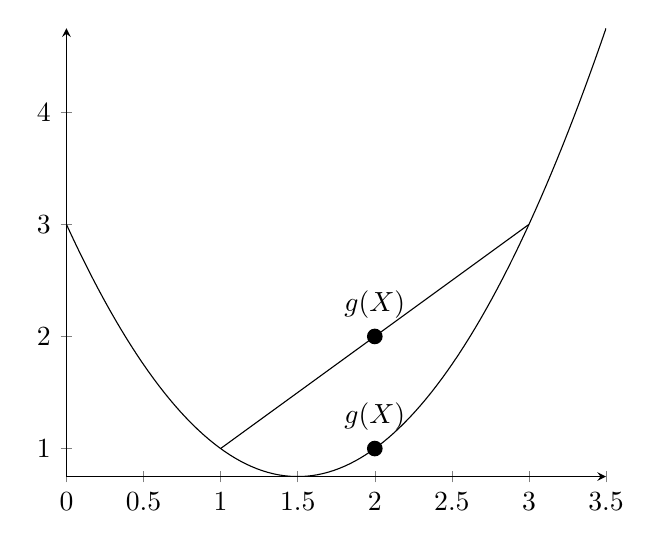
\begin{tikzpicture}
		\begin{axis} [
				axis lines = left,
			]
			\addplot [
				domain=0:3.5,
				samples=100,
			] {x^2 - 3*x + 3};

			\addplot [
				domain=1:3,
				samples=100,
			] {x};
			\node[label={90:{\(g(\E X)\)}},circle,fill,inner sep=2pt] at (axis cs:2,1) {};
			\node[label={90:{\(\E g(X)\)}},circle,fill,inner sep=2pt] at (axis cs:2,2) {};
		\end{axis}
	\end{tikzpicture}
	\caption{琴生不等式在\(g(x)=x^2-3x+3, \probP(X=1)=\probP(X=3)=1/2\)时的情况}
\end{figure}

\begin{theorem}[\textbf{赫尔德不等式(H\"older's inequality)}]
	\label{thm:1.6.3}
	若\(p,q\in\intcc{1,+\infty}\)满足\(1/p+1/q=1\),则
	\[\E\envert{XY}\leq\enVert{X}_p\enVert{Y}_q\]
	\(\enVert{X}_r:=\del{\E \envert{X}^r}^{1/r}, r\in\intco{1,+\infty}\),\(\enVert{X}_{+\infty}:=\inf\cbr{M:\probP\del{\envert{X}>M}=0}\)
\end{theorem}

在开始介绍下一个定理前,我们先引入一个记号,如果我们仅在某个\(A\subseteq \Omega\)上积分时,记作
\[\E(X;A):=\int_AX\,\dif\probP\]
\begin{theorem}[\term{切比雪夫不等式}(Chebyshev's inequality)] \label{thm:1.6.4}
	设函数\(\varphi:\R\mapsto\R\)非负,令\(A\in\mathcal{R}\)以及\(i_A=\inf\cbr{\varphi(y):y\in A}\),则有
	\[i_A\probP(X\in A)\leq\E(\varphi(X);X\in A)\leq\E\varphi(X)\]
\end{theorem}
\begin{proof}
	根据\(i_A\)的定义\(\varphi\)非负的条件,我们很容易得知
	\[i_A\indicator_{(A\in X)}\leq\varphi(X)\indicator_{(X\in A)}\leq\varphi(X)\]
	接着对上面的不等式求积分并根据\thmref{thm:1.6.1}的\ref{thm:1.6.1.3}即可。
\end{proof}
\begin{remark}
	有些作者称该不等式为\term{马尔科夫不等式}(Markov's inequality)并用切比雪夫不等式来称呼\(\varphi(x)=x^2\)且\(A=\cbr{x:\envert{x}\geq a}\)的情形:
	\begin{equation}
		a^2P(\envert{X}\geq a)\leq \E X^2
	\end{equation}
\end{remark}

\subsection{对极限积分}
下面我们将用期望的语言重新叙述之前的关于极限与积分何时能换序的相关内容。
\begin{theorem}[法图引理(Fatou's lemma)]
若随机变量列\(\sequence{X_n}_{n=1}\)中的通项\(X_n\geq0\)则
\[\liminf_{n\rightarrow+\infty}\E X_n\geq\E\del{\liminf_{n\rightarrow+\infty}X_n}\]
\end{theorem}
\begin{theorem}[单调收敛定理(Monotone convergence theorem)]
	若随机变量列\(\sequence{X_n}_{n=1}\)中的通项\(X_n\geq0\)且\(\lim\limits_{n\uparrow+\infty}X_n\stackrel{\uparrow}{=}X\),则\(\lim\limits_{n\uparrow+\infty}\E X_n\stackrel{\uparrow}{=}\E X\)。
\end{theorem}
\begin{theorem}[控制收敛定理(Dominated convergence theorem)]\label{thm:1.6.7}
	若随机变量列\(\sequence{X_n}_{n=1}\)满足\(X_n\xrightarrow{\text{a.s.}}X\)且通项均满足\(\envert{X_n}\leq Y\)且有\(\E Y<+\infty\),则\(\lim\limits_{n\rightarrow+\infty}\E X_n=\E X\)
\end{theorem}
\thmref{thm:1.6.7}中\(Y\)为常数的情形称为\textbf{有界收敛定理}。

随着学习的深入,我们需要推导一些其他关于极限与积分的性质,其中比较重要的情形有\(g(x)=\envert{x}^p,p>1\)和\(h(x)=x\)。
\begin{theorem}\label{thm:1.6.8}
	随机变量列\(\sequence{X_n}_{n=1}\)满足\(X_n\xrightarrow{\text{a.s.}}X\)。令连续函数\(g\)以及\(h\)满足:

	\begin{enumerate}
		\item \(g\geq0\),且\(\lim\limits_{\envert{x}\rightarrow+\infty}g(x)=+\infty\)。
		\item \(\lim\limits_{\envert{x}\rightarrow+\infty}\envert{h(x)}/g(x)=0\)
		\item \label{thm:1.6.8.3} 通项\(X_n\)满足\(\E g(X_n)\leq K<+\infty\)
	\end{enumerate}
	则\(\lim\limits_{n\rightarrow+\infty}\E h(X_n)=\E h(X)\)。
\end{theorem}
\begin{proof}
由于将\(h\)减去一常数不改变积分的收敛性,我们可以不失一般性地认为\(h(0)=0\)。选取一足够大的\(M\)使得只要\(\envert{x}\geq M\)就有\(P\del{\envert{X}=M}=0\)以及\(g(x)>0\)成立。
对任意随机变量\(Y\),定义\(\bar{Y}:=Y1_{\envert{Y}\leq M}\)。
那么从\(P\del{\envert{X}=M}=0\)我们可以得到\(\bar{X}_n\xrightarrow{\text{a.s.}}\bar{X}\)。由于\(h(\bar{X}_n)\)有界且\(h\)连续,那么根据\hyperref[thm:1.6.7]{有界收敛定理}就有
\label{eq:1.6.7(a)}
\begin{flalign*}
\text{(a)}&&\lim\limits_{n\rightarrow+\infty}\E(h(\bar{X}_n))&=\E(h(\bar{X}))&
\end{flalign*}
接下来控制``截断''带来的影响,根据:
\label{eq:1.6.7(b)}
\begin{flalign*}
\text{(b)}&&\envert{\E h(\bar{Y}) - \E h(Y)}\leq\E\envert{h(\bar{Y})-h(Y)}\leq\E(\envert{h(Y)};\envert{Y}>M)\leq\epsilon_M\E g(Y)&&
\end{flalign*}
其中\(\epsilon_M=\sup\cbr{\envert{h(x)}/g(x):\envert{x}\geq M}\)。第二个不等号成立是因为当\(\envert{Y}\leq M\)时\(\bar{Y}=Y\),并且我们还假定了\(h(0)=0\)。第三个不等号可以直接从\(\epsilon_M\)的定义得到。

令\hyperref[eq:1.6.7(b)]{(b)}中的\(Y=X_n\)并利用条件\ref{thm:1.6.8.3}便可得到
\label{eq:1.6.7(c)}
\begin{flalign*}
	\text{(c)}&&\envert{\E h(\bar{X}_n)-\E h(X_n)}&\leq K\epsilon_M&
\end{flalign*}
为了估计\(\envert{\E h(\bar{X})-\E h(X)}\),我们观察到\(g\)是非负连续的,因此根据\hyperref[thm:1.5.5]{法图引理}我们有
\[\E g(x)\leq\liminf_{n\rightarrow+\infty}\E g(X_n)\leq K\]
再令\hyperref[eq:1.6.7(b)]{(b)}中的\(Y=X\)便有
\label{eq:1.6.7(d)}
\begin{flalign*}
	\text{(d)}&&\envert{\E h(\bar{X})-\E h(X)}&\leq K\epsilon_M&
\end{flalign*}
利用三角不等式可以得到
\begin{multline*}
\envert{\E h(X_n) - \E h(X)} \leq \envert{\E h(X_n)-\E h(\bar{X}_n)}\\
+\envert{h(\bar{X}_n) - \E h(\bar{X})} + \envert{\E h(\bar{X}) - \E h(X)}
\end{multline*}
对上式取极限再利用\hyperref[eq:1.6.7(b)]{(a)}、\hyperref[eq:1.6.7(b)]{(c)}及\hyperref[eq:1.6.7(b)]{(d)}便有
\[\limsup_{n\rightarrow+\infty}\envert{\E h(X_n) - \E h(X)}\leq 2K\epsilon_M\]
然而我们有\(0\leq K<+\infty\)且\(\lim\limits_{M\rightarrow+\infty}\epsilon_M=0\)。
\end{proof}

\subsection{期望的计算}
尽管\((\Omega, \mathcal{F}, \probP)\)上的积分理论十分优雅,但是在实际应用的过程中我们还是希望将目光转移到能做微积分的空间上。因此在接下来的定理中\(S\)通常是\(\R^d\)

\begin{theorem}[换元公式]
\label{thm:1.6.9}
设\(X\)是\((S,\mathcal{S})\)上的随机元素,其分布为\(\mu\),即\(\mu(A) = \probP(X\in A)\)。
若\(f\)为从\((S,\mathcal{S})\)到\(\R, \mathcal{R}\)的可测函数,并满足\(f\geq0\)或\(\E\envert{f(X)}<+\infty\),则
\[\E f(X)=\int_Sf(y)\,\mu(\dif y)\]
\end{theorem}
\begin{remark}
至于为何称为换元公式,
记\(X\)为\(h\),那么\(\mu\)可以改写为\(\probP\circ h^{-1}\)
\[\int_{\Omega}f(h(\omega))\,\dif\probP=\int_Sf(y)\,\dif \,(\probP\circ h^{-1})\]
\end{remark}
\begin{proof}
为了证明该结果,我们考虑模仿\ref{sec:1.4}中积分的定义,将结果逐步推广到一般的可测函数上。读者应当对该方法引起重视,因为该方法会出现在后续章节的证明中。

\noindent\textit{情况一:指示函数.} 若\(B\in\mathcal{S}\)且\(f=\indicator_B\),利用积分的定义,则有
\[\E\indicator_B(X)=\probP(X\in B)=\mu(B)=\int_S\indicator_B(y)\mu(\dif y)\]

\noindent\textit{情况二:简单函数.}令\(f(x)=\sum_{m=1}^nc_m\indicator_{B_m}(x)\),其中\(c_m\in\R, B_m\in\mathcal{S}\)。根据期望的线性性、情况一的结果以及积分的线性我们可以得到
\[\begin{split}
	\E f(X)=&\sum_{m=1}^nc_m\E \indicator_{B_m}(X)\\
	=&\sum_{m=1}^nc_m\int_S \indicator_{B_m}(y)\mu(\dif y)=\int_Sf(y)\mu(\dif y)
\end{split}\]

\noindent\textit{情况三:非负函数.}若\(f\geq0\),定义
\[f_n(x)=([2^nf(x)]/2^n)\wedge n\]
其中\([x]\)为\hyperlink{https://zh.wikipedia.org/zh-hans/取整函数}{取整函数},\(a\wedge b=\min\cbr{a,b}\),那么容易验证\(f_n\)是简单函数,而且\(\lim\limits_{n\uparrow+\infty}f_n \stackrel{\uparrow}{=} f\)。根据上一情况的结论并结合\hyperref[thm:1.5.5]{单调收敛定理}便有
\[\E f(X)=\lim_{n\rightarrow+\infty}\E f_n(X)=\lim_{n\rightarrow+\infty}\int_Sf_n(y)\mu(\dif y)
=\int_Sf(y)\mu(\dif y)\]

\noindent\textit{情况四:可积函数.}至于该情况,只需要把\(f\)写成\(f(x)=f(x)^+-f(x)^-\)即可。\(\E\envert{f(X)}<+\infty\)保证了\(\E f(X)^+\)和\(\E f(X)^-\)均有限。因此利用在非负函数情况下得到的结论配合积分的线性性便可得到
\[\begin{split}
	\E f(X)=\E f(X)^+ - \E f(X)^-=&\int_S f(y)^+\mu(\dif y)-\int_S f(y)^-\mu(\dif y)\\
	=&\int_S f(y)\mu(\dif y)
\end{split}\]
四种情况均已验证,证毕。
\end{proof}
有了\ref{thm:1.6.9}后,我们就可以将随机变量期望的计算问题转变为实直线上的积分问题。在展示例子前,先介绍一些术语。若\(k\)为一正整数,称\(\E X^k\)为\(X\)的\term{\(k\)-阶矩},我们通常称一阶矩\(\E X\)为\term{均值}并记作\(\mu\)。如果\(\E X^2<+\infty\),那么定义\(X\)的\term{方差}为\(\Var(X)=\E(X-\mu)^2\)。
通常公式
\begin{equation}\begin{split}
	\Var(X)=&\E(X-\mu)^2\\
	=&\E X^2-2\mu\E X+\mu^2=\E X^2-\mu^2
\end{split}\end{equation}
可以起到简化计算的作用。
从上式我们可以立即得出
\begin{equation}
	\Var(X)\leq \E X^2
\end{equation}
这里\(\E X^2\)表示\(X^2\)的期望。为了不引起混淆我们会把\(\E X\)的平方记作\((\E X)^2\)。
利用\hyperref[thm:1.6.1.2]{定理1.6.1(b)}可知\(\E(aX+b)=a\E X + b\),然后根据方差的定义我们可以立刻得到
\begin{equation} \label{eq:1.6.4}
\begin{split}
	\Var(aX+b)=&\E(aX+b-\E(aX+b))^2\\
	=&a^2\E(X-\E X)^2=a^2\Var(X)
\end{split}
\end{equation}
现在我们可以将目光放到一些例子上了,前两个例子中的计算细节由读者自行完成(用分部积分法)。
\begin{example}
若\(X\)服从率参数为\(1\)的\term{指数分布(exponential distribution)}则其\(k\)-阶矩为
\[\E X^k=\int_0^{+\infty}x^ke^{-x}\dif x=k!\]
所以\(X\)得均值是\(1!=1\),方差是\(\E X^2-(\E X)^2=2!-1^2=1\)。如果令\(Y=X/\lambda\),利用\ref{exe:1.2.5}就可以知道\(Y\)的指数分布的概率密度函数为\(\lambda e^{-\lambda y},y\geq0\)即率参数为\(\lambda\)的\term{指数密度(exponential density)}。
再利用\autoref{thm:1.6.1}\ref{thm:1.6.1.2}和(\ref{eq:1.6.4}),便可知\(Y\)的均值为\(1/\lambda\),方差为\(1/\lambda^2\)。
\end{example}
\begin{example}
若\(X\)服从\term{标准正态分布},根据对称性可知
\[\E X=\int_{\R}x\frac{1}{\sqrt{2\pi}}e^{-\frac{x^2}{2}}=0\]
\[\Var(X)=\E X^2=\int_{\R}x^2\frac{1}{\sqrt{2\pi}}e^{-\frac{x^2}{2}}=1\]
如果令\(\sigma>0,\mu\in\R\),做换元\(Y=\sigma X+\mu\)再利用\autoref{thm:1.6.1}\ref{thm:1.6.1.2}和(\ref{eq:1.6.4}),便可知\(Y\)的概率密度为
\[\frac{1}{\sqrt{2\pi\sigma^2}}e^{-\frac{(y-\mu)^2}{2}}\]
即均值为\(\mu\),方差为\(\sigma^2\)的\term{正态分布}。
\end{example}
接下来我们将考虑一些离散分布。其中第一种是最为简单的,但在后文中起到了不少作用,故首先介绍。
\begin{example}
	称\(X\)服从参数为\(p\)的\term{伯努利分布(Bernoulli distribution)},若\(P(X=1)=p\)且\(P(X=0)=1-p\)。
	显然,
	\[\E X=p\cdot 1+(1-p)\cdot 0=p\]
	由于\(X^2=X\),故\(\E X^2=\E X=p\)所以
	\[\Var(X)=\E X^2-(\E X)^2=p-p^2=p(1-p)\]
\end{example}
\begin{example}
	称\(X\)服从强度为\(\lambda\)的\term{泊松分布(Poisson distribution)},若对非负整数\(k\)有
	\[P(X=k)=e^{-\lambda}\lambda^k/k!\]
	为了求出\(X\)的矩,我们只需``注意到''
	对\(k\geq1\)有
	\[\begin{split}
		\E(X(X-1)\cdots(X-k+1))=&\sum_{j=k}^{+\infty}j(j-1)\cdots(j-k+1)e^{-\lambda}\frac{\lambda^j}{j!}\\
		=&\lambda^k\sum_{j=k}^{+\infty}e^{-\lambda}\frac{\lambda^{j-k}}{(j-k)!}=\lambda^k
	\end{split}\]
	该等式之所以成立是因为
	\begin{enumerate*}
		\item \(j(j-1)\cdots(j-k+1)\)在\(j<k\)时为0
		\item 消去了部分阶乘中的因子
		\item 泊松分布的总质量为\(1\)
	\end{enumerate*}
	因此根据上述式子,我们有\(\E X=\lambda\)同时
	\[\Var(X)=\E X^2-(\E X)^2=\E(X(X-1))+\E X-\lambda^2=\lambda\]
\end{example}
\begin{example}
	称\(N\)服从成功率为\(p\intoo{0,1}\)的几何分布,若对正整数\(k\)
	\[P(N=k)=p(1-p)^{k-1}\]
	所以\(N\)做独立且重复的试验,直到观测到事件成功的试验次数。
	注意到
	\[\sum_{k=1}^{+\infty}p(1-p)^{k-1}=1\Rightarrow\sum_{k=0}^{+\infty}(1-p)^{k}=1/p\]
\end{example}
对其取微分并借助\ref{exp:a.5.6}可知
\[-\sum_{k=1}^{+\infty}k(1-p)^{k-1}=-1/p^2\]
\[\sum_{k=2}^{+\infty}k(k-1)(1-p)^{k-2}=2/p^3\]
由此可知
\[\E N=\sum_{k=1}^{+\infty}kp(1-p)^{k-1}=1/p\]
\[\E N(N-1)=\sum_{k=1}^{+\infty}k(k-1)p(1-p)^{k-1}=2(1-p)/p^2\]
\[\begin{split}
	\Var(N)=&\E N^2-(\E N)^2=\E N(N-1)+\E N-(\E N)^2\\
	=&\frac{2(1-p)}{p^2}+\frac{p}{p^2}-\frac{1}{p^2}
	=\frac{1-p}{p^2}
\end{split}\]
\section*{习题}
\begin{exercise}
\item 设\(\varphi\)严格凸,即\(>\)对任意\(\lambda\in\intoo{0,1}\)成立。证明在\ref{thm:1.6.2}的假设下,\(\varphi(\E X)=\E\varphi(X)\)蕴含\(X=\E X\) a.s.
\item 设\(\varphi:\R^n\mapsto\R\)凸,通过模仿\ref{thm:1.5.1}的证明来说明若\(\E\envert{\varphi(X_1,\dots,X_n)}<+\infty\)且\(\E\envert{X_i}<+\infty\)对所有\(i\)均成立,则
\[\E\varphi(X_1,\dots,X_n)\geq\varphi(\E X_1,\dots,\E X_n)\]
\item \textbf{切比雪夫不等式的改进空间}
(i)通过证明:如果对于固定的\(0<b\leq a\),存在\(X\)使得\(\E X^2=b^2\)且有\(\probP(\envert{X}\geq a)=b^2/a^2\)。来证明此时\autoref{thm:1.6.4}不存在改进空间
(ii)通过证明:如果\(X\)满足\(0<\E X^2<+\infty\),则
\[\lim\limits_{a\rightarrow+\infty}a^2\probP(\envert{X}\geq a)/\E X^2=0\]
来证明此时\ref{thm:1.6.4}给出的界存在改进空间。

\item \textbf{切比雪夫不等式的单边界}
(i) 给定\(a>b>0,0<p<1\),并令随机变量\(X\)满足\(\probP(X=a)=p,\probP(X=b)=1-p\),在\autoref{thm:1.6.4}中令\(\varphi(x)=(x+b)^2\)来说明对任意满足\(\E Y=\E X, \Var(Y)=\Var(X)\)的r.v.\(Y\)均有\(\probP(Y\geq a)\leq p\)且在\(Y=X\)时取到等号。
(ii) 设\(\E Y=0,\Var(Y)=\sigma^2,a>0\)。证明\(\probP(Y\geq a)\leq \sigma^2/(a^2+\sigma^2)\),且存在\(Y\)使得等号成立。
\item \textbf{两个不存在的下界}\\
证明:(i) 若\(\epsilon>0\)则\(\inf\cbr{\probP(\envert{X}>\epsilon):\E X=0,\Var(X)=1}=0\)。
(ii)若\(y\geq1, \sigma^2\intoo{0,+\infty}\),则\(\inf\cbr{\probP(\envert{X}>y):\E X=0,\Var(X)=\sigma^2}=0\)。
\item \textbf{一个常用下界}令r.v.\(Y\)满足\(\E Y=0,\E Y^2<+\infty\)。对\(Y\indicator_{Y>0}\)使用\hyperref[thm:1.5.2]{柯西--施瓦茨不等式}导出
\[\probP(Y>0)\geq (\E Y)^2/\E Y^2\]
\item 令\(\Omega=\intoo{0,1}\),并配备其上的博雷尔集以及勒贝格测度构成测度空间。令\(\alpha\in\intoo{1,2}\)且定义\(X_n=n^{\alpha}\indicator_{\intoo{1/(n+1),1/n}}\)并满足\(\lim_{n\rightarrow+\infty}X_n=0 \text{ a.s.}\)。说明可以在\autoref{thm:1.6.8}中令\(h(x)=x,g(x)=\envert{x}^{2/\alpha}\),但\(X_n\)不被任何可积函数控制。
\item 设概率测度\(\mu\)满足\(\forall A\in\mathcal{R}, \mu(A)=\int_Af(x)\dif x\)。利用\autoref{thm:1.6.9}的证明方法证明对任意满足\(g\geq0\)或\(\int \envert{g(x)}\mu(\dif x)<+\infty\)的函数\(g\)有
\[\int g(x)\mu(\dif x)=\int g(x)f(x)\dif x\]
\item \term{容斥原理} 令\(A_1,A_2,\dots,A_n\)为事件,\(A=\cup_{i=1}^nA_i\)。
证明\(\indicator_A=1-\prod_{i=1}^n(1-\indicator_{A_{i}})\),展开等号右侧并取期望得出
\[\begin{split}
	\probP\del{\bigcup_{i=1}^n A_i}=&\sum_{i=1}^n\probP(A_i)-\sum_{i<j}\probP(A_i\cap A_j)\\
	+&\sum_{i<j<k}\probP(A_i\cap A_j\cap A_k)-\dots+(-1)^{n-1}\probP\del{\bigcap_{i=1}^nA_i}
\end{split}\]
\item \term{邦费罗尼不等式(Bonferroni inequalities)}
令\(A_1,A_2,\dots,A_n\)为事件,\(A=\cup_{i=1}^nA_i\)。
证明
\begin{align*}
	\indicator_A\leq&\sum_{i=1}^n\indicator_{A_i}\\
	\indicator_A\geq&\sum_{i=1}^n\indicator_{A_i}-\sum_{i<j}\indicator_{A_i}\cdot1_{A_j}\\
	\indicator_A\leq&\sum_{i=1}^n\indicator_{A_i}-\sum_{i<j}\indicator_{A_i}\cdot1_{A_j}+\sum_{i<j<k}\indicator_{A_i}\cdot1_{A_j}\cdot 1_{A_k}\\
	\vdots&
\end{align*}
取期望得到
\begin{align*}
	\probP(A)\leq&\sum_{i=1}^n\probP(A_i)\\
	\probP(A)\geq&\sum_{i=1}^n\probP(A_i)-\sum_{i<j}\probP(A_i\cap A_j)\\
	\probP(A)\leq&\sum_{i=1}^n\probP(A_i)-\sum_{i<j<k}\probP(A_i\cap A_j)+\sum_{i<j}\probP(A_i\cap A_j\cap A_k)\\
	\vdots&
\end{align*}
一般地,如果我们在容斥原理中保留偶(奇)数项,可以得到一个不等式下(上)界。
\item 若\(\E \envert{X}^k<+\infty\),那么对于\(0<j<k\)有\(\E \envert{X}^j<+\infty\),进一步地,我们还有
\[\E\envert{X}^j\leq(\E \envert{X}^k)^{j/k}\]
\item 在\hyperref[thm:1.6.2]{琴生不等式}中令\(\varphi(x)=e^x\)以及\(\probP(X=\log y_m)=p(m)\)继而证明
若\(\sum_{m=1}^np(m)=1\)且\(p(m),y_m>0\)则
\[\sum_{m=1}^np(m)y_m\geq\prod_{m=1}^ny_m^{p(m)}\]
当\(p(m)=1/n\)时,该不等式称为均值不等式。
\item 若\(\E X_1^-<+\infty\)且\(\lim_{n\uparrow+\infty}X_n\stackrel{\uparrow}{=}X\)则\(\lim_{n\uparrow+\infty}\E X_n\stackrel{\uparrow}{=}\E X\)。
\item 令\(X\geq0\)但\textbf{不假定}\(\E (1/X)<+\infty\),证明
\[\lim\limits_{y\rightarrow+\infty}y\E(1/X;X>y)=0\]
\[\lim\limits_{y\downarrow 0}y\E(1/X;X>y)=0\]
\item 若\(X_n\geq 0\)则\(\E\del{\sum_{n=1}^{+\infty}X_n}=\sum_{n=1}^{+\infty}\E X_n\)。
\item 若\(X\)可积,\(\sequence{A_n}_{n=0}\)为互不相交的集合列且\(\bigcup_{n=1}^{+\infty}A_n=A\),则有
\[\sum_{n=0}^{+\infty}\E(X;A_n)=\E(X;A)\]
即等号左侧的和式绝对收敛,且收敛到等号右侧的值。
\end{exercise}

\section{积测度、富比尼定理} \label{sec:1.7}
\begin{theorem}
\label{thm:1.7.2}
\end{theorem}
\begin{exercise}
	\item
	\item
	\item
	\item \label{e1.7.4}
\end{exercise}
\end{document}
